\documentclass[a4paper,11pt]{book}
\usepackage{listings}
\usepackage[utf8]{inputenc}
\usepackage[english]{babel}


\hfuzz=30pt % Suppress overfull warnings.
%\decimalpoint
\usepackage{dcolumn}
\newcolumntype{.}{D{.}{\esperiod}{-1}}
\makeatletter
\addto\shorthandsspanish{\let\esperiod\es@period@code}
\makeatother


%\usepackage[chapter]{algorithm}
\RequirePackage{verbatim}
\usepackage{fancyhdr}
\usepackage{graphicx}
\usepackage{afterpage}

\usepackage{longtable}

%\usepackage[pdfborder={000}]{hyperref} %referencia
\usepackage{hyperref} %referencia

% ********************************************************************
% Re-usable information
% ********************************************************************
\newcommand{\myTitle}{Título del proyecto\xspace}
\newcommand{\myDegree}{Master Universitario en Ingeniería de Teñe3comunicación\xspace}
\newcommand{\myName}{Nombre Apllido1 Apellido2 (alumno)\xspace}
\newcommand{\myProf}{Nombre Apllido1 Apellido2 (tutor1)\xspace}
\newcommand{\myOtherProf}{Nombre Apllido1 Apellido2 (tutor2)\xspace}
\newcommand{\mySupervisor}{Put name here\xspace}
\newcommand{\myFaculty}{Escuela Técnica Superior de Ingenierías Informática y de
Telecomunicación\xspace}
\newcommand{\myFacultyShort}{E.T.S. de Ingenierías Informática y de
Telecomunicación\xspace}
\newcommand{\myDepartment}{Departamento de ...\xspace}
\newcommand{\myUni}{\protect{Universidad de Granada}\xspace}
\newcommand{\myLocation}{Granada\xspace}
\newcommand{\myTime}{\today\xspace}
\newcommand{\myVersion}{Version 0.1\xspace}


\hypersetup{
pdfauthor = {\myName (email (en) ugr (punto) es)},
pdftitle = {\myTitle},
pdfsubject = {},
%pdfkeywords = {palabra_clave1, palabra_clave2, palabra_clave3, ...},
pdfcreator = {LaTeX con el paquete ....},
pdfproducer = {pdflatex}
}

%%%%%%%%%%% PACKAGES ADDED BY ME %%%%%%%%%%%%%%%%%%%%%%%%%%%%%%%%%%%%%%%%%%%
\usepackage[nottoc]{tocbibind}  % Include the bibliography in the ToC.
\usepackage{url}
\usepackage{listings} % To format code.
\usepackage{float} % Use [H] tag on figures.
\usepackage[table,x11names,pdftex,dvipsnames]{xcolor} % Table colors.
\usepackage{eurosym} % Euro symbol.
\usepackage[binary-units]{siunitx} % Proper spacing between units and values.
\usepackage[toc,page]{appendix}  % Enable appendices.
\usepackage[toc,nonumberlist]{glossaries}  % Glossary.
%%%%%%%%%%%%%%%%%%%%%%%%%%%%%%%%%%%%%%%%%%%%%%%%%%%%%%%%%%%%%%%%%%%%%%%%%%%%

\usepackage{colortbl,longtable}
\usepackage[stable]{footmisc}


%%%%%%%%%%%%%
\usepackage[colorinlistoftodos,prependcaption,textsize=footnotesize]{todonotes}

%\usepackage[pdftex,dvipsnames]{xcolor}  % Coloured text etc.
\usepackage{xargs}                      % Use more than one optional parameter in a new commands

\newcommandx{\cjorge}[2][1=]{\todo[inline,linecolor=purple,backgroundcolor=purple!25,bordercolor=purple,#1]{Jorge: #2}}
\newcommandx{\cangel}[2][1=]{\todo[inline,linecolor=orange,backgroundcolor=orange!25,bordercolor=orange,#1]{Ángel:: #2}}

% ********************************************************************
% 							GLOSSARY
% ********************************************************************
\makeglossaries
\newacronym{advisor}{ADVisor}{ADvanced Flowvisor}
\newacronym{api}{API}{Application Programming Interface}
\newacronym{arp}{ARP}{Address Resolution Protocol}
\newacronym{bpg}{BGP}{Border Gateway Protocol}
\newacronym{bsd}{BSD}{Berkeley Software Distribution}
\newacronym{cli}{CLI}{Command Line Interface}
\newacronym{cpu}{CPU}{Central Processing Unit}
\newacronym{diffserv}{DiffServ}{Differentiated Services}
\newacronym{dpid}{DPID}{Datapath Identifier}
\newacronym{dscp}{DSCP}{Differentiated Services Code Point}
\newacronym{glbp}{GLBP}{Gateway Load Balancing Protocol}
\newacronym{gpg}{GPG}{GNU Privacy Guard}
\newacronym{gnu}{GNU}{GNU is Not Unix}
\newacronym{gui}{GUI}{Graphical User Interface}
\newacronym{hsrp}{HSRP}{Hot Standby Router Protocol}
\newacronym{icmp}{ICMP}{Internet Control Message Protocol}
\newacronym{io}{IO}{Input OutpPut}
\newacronym{ip}{IP}{Internet Protocol}
\newacronym{ipfix}{IPFIX}{IP Flow Information Export}
\newacronym{iot}{IoT}{Internet of Things}
\newacronym{jit}{JIT}{Just In Time}
\newacronym{lacp}{LACP}{Link Aggregation Control Protocol}
\newacronym{lan}{LAN}{Local Area Network}
\newacronym{lora}{LoRa}{Long Range}
\newacronym{lorawan}{LoRaWAN}{LoRa Wide Area Network}
\newacronym{lts}{LTS}{Long Term Support}
\newacronym{netconf}{NETCONF}{Network Configuration Protocol}
\newacronym{netflow}{NetFlow}{Network Flow}
\newacronym{mac}{MAC}{Media Access Control}
\newacronym{mpls}{MPLS}{MultiProtocol Label Switching}
\newacronym{mqtt}{MQTT}{Message Queue Telemetry Transport}
\newacronym{oasis}{OASIS}{Organization for the Advancement of Structured Information Standards}
\newacronym{os}{OS}{Operative System}
\newacronym{ospf}{OSPF}{Open Shortest Path First}
\newacronym{ovs}{OVS}{Open vSwitch}
\newacronym{qemu}{QEMU}{Quick Emulator}
\newacronym{qos}{QoS}{Quality of Service}
\newacronym{rspan}{RSPAN}{Remote Switched Port Analyzer}
\newacronym{sdn}{SDN}{Software Defined Network}
\newacronym{sflow}{sFlow}{sampled Flow}
\newacronym{snmp}{SNMP}{Simple Network Management Protocol}
\newacronym{snr}{SNR}{Signal to Noise Ratio}
\newacronym{ssh}{SSH}{Secure Shell}
\newacronym{tcp}{TCP}{Transmission Control Protocol}
\newacronym{tos}{ToS}{Type of Service}
\newacronym{rest}{REST}{Representational State Transfer}
\newacronym{rip}{RIP}{Routing Information Protocol}
\newacronym{udp}{UDP}{User Datagram Protocol}
\newacronym{vat}{VAT}{Value Added Tax}
\newacronym{vertigo}{VeRTIGO}{ViRtual TopologIes Generalization in Openflow}
\newacronym{vlan}{VLAN}{Virtual LAN}


\pagestyle{fancy}
\fancyhf{}
\fancyhead[LO]{\leftmark}
\fancyhead[RE]{\rightmark}
\fancyhead[RO,LE]{\textbf{\thepage}}
\renewcommand{\chaptermark}[1]{\markboth{\textbf{#1}}{}}
\renewcommand{\sectionmark}[1]{\markright{\textbf{\thesection. #1}}}

\setlength{\headheight}{1.5\headheight}

\newcommand{\HRule}{\rule{\linewidth}{0.5mm}}
%Definimos los tipos teorema, ejemplo y definición podremos usar estos tipos
%simplemente poniendo \begin{teorema} \end{teorema} ...
\newtheorem{teorema}{Teorema}[chapter]
\newtheorem{ejemplo}{Ejemplo}[chapter]
\newtheorem{definicion}{Definición}[chapter]

\definecolor{gray97}{gray}{.97}
\definecolor{gray75}{gray}{.75}
\definecolor{gray45}{gray}{.45}
\definecolor{gray30}{gray}{.94}

\lstset{ frame=Ltb,
     framerule=0.5pt,
     aboveskip=0.5cm,
     framextopmargin=3pt,
     framexbottommargin=3pt,
     framexleftmargin=0.1cm,
     framesep=0pt,
     rulesep=.4pt,
     backgroundcolor=\color{gray97},
     rulesepcolor=\color{black},
     %
     stringstyle=\ttfamily,
     showstringspaces = false,
     basicstyle=\scriptsize\ttfamily,
     commentstyle=\color{gray45},
     keywordstyle=\bfseries,
     %
     numbers=left,
     numbersep=6pt,
     numberstyle=\tiny,
     numberfirstline = false,
     breaklines=true,
   }

% minimizar fragmentado de listados
\lstnewenvironment{listing}[1][]
   {\lstset{#1}\pagebreak[0]}{\pagebreak[0]}

\lstdefinestyle{CodigoC}
   {
	basicstyle=\scriptsize,
	frame=single,
	language=C,
	numbers=left
   }
\lstdefinestyle{CodigoC++}
   {
	basicstyle=\small,
	frame=single,
	backgroundcolor=\color{gray30},
	language=C++,
	numbers=left
   }


\lstdefinestyle{Consola}
   {basicstyle=\scriptsize\bf\ttfamily,
    backgroundcolor=\color{gray30},
    frame=single,
    numbers=none
   }


\newcommand{\bigrule}{\titlerule[0.5mm]}


%Para conseguir que en las páginas en blanco no ponga cabecerass
\makeatletter
\def\clearpage{%
  \ifvmode
    \ifnum \@dbltopnum =\m@ne
      \ifdim \pagetotal <\topskip
        \hbox{}
      \fi
    \fi
  \fi
  \newpage
  \thispagestyle{empty}
  \write\m@ne{}
  \vbox{}
  \penalty -\@Mi
}
\makeatother

\usepackage{pdfpages}

\begin{document}
\begin{titlepage}

\newlength{\centeroffset}
\setlength{\centeroffset}{-0.5\oddsidemargin}
\addtolength{\centeroffset}{0.5\evensidemargin}
\thispagestyle{empty}

\noindent\hspace*{\centeroffset}\begin{minipage}{\textwidth}

\centering

\includegraphics[width=0.9\textwidth]{imagenes/logo_ugr.jpg}\\[1.4cm]

\textsc{\Large MASTER THESIS\\[0.2cm]}
\textsc{TELECOMMUNICATIONS ENGINEERING}\\[1cm]
% Upper part of the page
%
% Title
{\Huge\bfseries SDN Based Network Slicing\\
}
%\noindent\rule[-1ex]{\textwidth}{3pt}\\[3.5ex]
%{\large\bfseries Subtitulo del Proyecto}
\end{minipage}

\vspace{2.5cm}
\noindent\hspace*{\centeroffset}\begin{minipage}{\textwidth}
\centering

\textbf{Author}\\ {Angel Guzman-Martinez}\\[2.5ex]
\textbf{Supervisor}\\
{Jorge Navarro-Ortiz}\\[2cm]

\includegraphics[width=0.3\textwidth]{imagenes/etsiit_logo.png}\\[0.1cm]
\textsc{School of Informatics and Telecommunications Engineering}\\
\textsc{---}\\
Granada, June of 2019
\end{minipage}
%\addtolength{\textwidth}{\centeroffset}
%\vspace{\stretch{2}}
\end{titlepage}




\chapter*{}
\begin{titlepage}
 
 
\setlength{\centeroffset}{-0.5\oddsidemargin}
\addtolength{\centeroffset}{0.5\evensidemargin}
\thispagestyle{empty}

\noindent\hspace*{\centeroffset}\begin{minipage}{\textwidth}

\centering
%
\includegraphics[width=0.9\textwidth]{imagenes/logo_ugr.jpg}\\[1.4cm]

%\textsc{ \Large PROYECTO FIN DE CARRERA\\[0.2cm]}
%\textsc{ INGENIERÍA EN INFORMÁTICA}\\[1cm]
% Upper part of the page
% 

 \vspace{3.3cm}

%si el proyecto tiene logo poner aquí
%
\includegraphics{imagenes/logo.png} 
% \vspace{0.5cm}

% Title

{\Huge\bfseries SDN Based Network Slicing\\
}
%\noindent\rule[-1ex]{\textwidth}{3pt}\\[3.5ex]
%{\large\bfseries Subtítulo del proyecto.\\[4cm]}
\end{minipage}

\vspace{2.5cm}
\noindent\hspace*{\centeroffset}\begin{minipage}{\textwidth}
\centering

\textbf{Author}\\ {Angel Guzman-Martinez}\\[2.5ex]
\textbf{Supervisor}\\
{Jorge Navarro-Ortiz}\\[2cm]

\includegraphics[width=0.15\textwidth]{imagenes/tstc.png}\\[0.1cm]
\textsc{Dpt. of Signal Theory, Telematics and Communications}\\
\textsc{---}\\
Granada, July of 2019
\end{minipage}
%\addtolength{\textwidth}{\centeroffset}
\vspace{\stretch{2}}

 
\end{titlepage}





\cleardoublepage
\thispagestyle{empty}

\begin{center}
{\large\bfseries Particionado de Red Basado en Redes SDN}\\
\end{center}
\begin{center}
Ángel Guzmán Martínez\\
\end{center}

%\vspace{0.7cm}
\noindent{\textbf{Palabras clave}:  hipervisor, particionado de red, SDN, tráfico heterogéneo.}\\

\vspace{0.7cm}
\noindent{\textbf{Resumen}}\\

Hoy en día, las diferentes redes desplegadas alrededor del mundo tienen que lidiar con tráfico muy heteroǵeneo. Esto se acentúa más aún con la introducción del Internet de las Cosas. Especialmente con la llegada del 5G en un futuro próximo, las redes celulares tendrán que tratar con diferentes flujos de tráfico cuyas necesidades de ancho de banda difieren en gran medida.

Tradicionalmente, para dar un trato especializado a diferentes flujos de tráfico se aplican técnicas de \textit{Quality of Service} (QoS). Dichas técnicas permiten a las redes distinguir entre diferentes tipos de paquetes y aplicarles políticas distintas. 

No obstante, el uso de mecanismos de QoS, como \textit{DiffServ} que es la implementación más habitual, tiene sus limitaciones. Por ejemplo, no es posible aplicar ingeniería de tráfico sino que se basa en el uso de prioridades. Es decir, los paquetes prioritarios viajan junto al resto del tráfico, pero son procesados antes por los \textit{routers} y pasan menos tiempo en colas. 

Para aplicar ingeniería de tráfico, habría que hacer uso de otros protocolos como MPLS. A su vez, MPLS tiene también sus desventajas. Requiere que los \textit{routers} tengan capacidades adicionales y tiene carencias de flexibilidad y adaptabilidad.

Una de las posibles soluciones a este problema consiste en particionar Redes Definidas por \textit{Software} (SDN), ya que esta técnica ofrece la posiblidad de separar flujos de datos del mismo tipo de tráfico. No obstante, esta tecnología es relativamente reciente y no está lo suficientemente madura y, en consecuencia, presenta algunos problemas en su implementación.

En el presente proyecto plantea la exploración del uso de un hipervisor en SDN para simplificar el particionado de la red. Al mismo tiempo, usar un hipervisor solventa, o al menos palia, los inconvenientes que presenta el método covencional de redes SDN sin hipervisor, especialmente la escalabilidad, flexibilidad y adaptabilidad.

\cleardoublepage


\thispagestyle{empty}


\begin{center}
{\large\bfseries SDN Based Network Slicing}\\
\end{center}
\begin{center}
Angel Guzman-Martinez\\
\end{center}

%\vspace{0.7cm}
\noindent{\textbf{Keywords}: heterogeneous traffic, hypervisor, network slicing, SDN.}\\

\vspace{0.7cm}
\noindent{\textbf{Abstract}}\\

Nowadays, the different networks deployed around the world have to handle very heterogeneous traffic. Even more so with the introduction of the Internet of Things. Furthermore, with the arrival of 5G in the near future, cell networks will have to deal with different types of traffic whose bandwidth needs vary widely.

Traditionally, in order to treat each type of traffic in a different manner, Quality of Service (QoS) techniques are applied. These techniques allow networks to distinguish between different types of packets and apply different policies to each type.

However, QoS techniques, such as DiffServ which is the most common implementation, have some limitations. For instance, it is not possible to apply traffic engineering, it relies on the use of priorities instead. This means the high priority packets are routed with the rest of the traffic, but they are processed faster and spend less time waiting in queues. 

To perform traffic engineering, other protocols, such as MPLS, need to be used. Likewise, MPLS has its own drawbacks. It requires routers with additional capabilities and lacks flexibility and adaptability.

One of the possible solutions involves slicing Software Defined Networks (SDN). Yet, this technology is relatively recent and is not mature enough. Consequently, there are some implementation issues.

As a result, the present project proposes to explore the use of hypervisor within SDN, in order to simplify network slicing while solving, or at least diminishing, the pitfalls of a conventional SDN without hypervisor, i.e., scalibility, flexibility and adaptability.

\chapter*{}
\thispagestyle{empty}

\noindent\rule[-1ex]{\textwidth}{2pt}\\[4.5ex]

Yo, \textbf{Ángel Guzmán Martínez}, alumno de la titulación Máster Universitario en Ingeniería de Telecomunicación de la \textbf{Escuela Técnica Superior de Ingenierías Informática y de Telecomunicación de la Universidad de Granada}, con DNI 75573604, autorizo la ubicación de la siguiente copia de mi Trabajo Fin de Master en la biblioteca del centro para que pueda ser consultada por las personas que lo deseen.

\vspace{6cm}

\noindent Fdo: Ángel Guzmán Martínez

\vspace{2cm}

\begin{flushright}
Granada, julio de 2019.
\end{flushright}


\chapter*{}
\thispagestyle{empty}

\noindent\rule[-1ex]{\textwidth}{2pt}\\[4.5ex]

D. \textbf{Jorge Navarro Ortiz}, Profesor Titular de Universidad del Área de Ingeniería Telemática del Departamento de Teoría de la Señal, Telemática y Comunicaciones de la Universidad de Granada.

\vspace{0.5cm}

\textbf{Informa:}

\vspace{0.5cm}

Que el presente trabajo, titulado \textit{\textbf{SDN Based Network Slicing}}, ha sido realizado bajo su supervisión por \textbf{Ángel Guzmán Martínez}, y autorizo la defensa de dicho trabajo ante el tribunal que corresponda.

\vspace{0.5cm}

Y para que conste, expide y firma el presente informe en Granada a 27 de junio de 2019.

\vspace{1cm}

\textbf{Los directores:}

\vspace{5cm}

\noindent \textbf{Jorge Navarro Ortiz \ \ \ \ \ }

\chapter*{Acknowledgements}
\thispagestyle{empty}

       \vspace{1cm}


Thanks to Jorge, he is such a nice, hardworking person and always willing to help. Although, because of this, he is also very busy most of the time. He also accepted to supervise my thesis despite me asking a little bit late.

Thanks to Juanma, for lending us a USB-Ethernet adapter in times of need. Great person as well, always offering advice.

Also thanks to my friends, for constantly nagging me about how my thesis is going. While annoying at the time, it helped me stay motivated to finish it so that they would shut up about it. 


\frontmatter
\pagenumbering{Roman}  % Use uppercase roman numbers.
\tableofcontents
\listoffigures
\listoftables
\glsaddall
\printglossaries

\mainmatter
\setlength{\parskip}{5pt}
\chapter{Introduction} \label{chapter:introduction}

\section{Context and Motivation}
The world of telecommunications is evolving. Every so often there is a new network protocol, technique or application. A recent one that is gaining a lot of traction is the Internet of Things (IoT), which will have proper support in the coming generation of cell networks, in addition to other new protocols such as enhanced mobile broadband (eMBB) and ultra-reliable low latency communications (URLLC).

With such heterogeneous traffic being handled by the network, it is not efficient to treat everything equally, as each type of traffic has its own needs. For instance, traffic coming from an IoT device usually does not need much bandwidth whatsoever. As a result, there is a need to distinguish between different types of traffic so that each one can be treated accordingly.  

The old fashioned solution to this problem would be to apply QoS techniques, based on priorities, or traffic engineering protocols such as MPLS. However, both alternatives suffer from some limitations.
\begin{itemize}
    \item DiffServ, currently the most common implementation of QoS, works time with aggregated traffic. This means that it cannot distinguish between two tenants sending the same type of traffic.
    \item DiffServ and MPLS both require that the network implements additional capabilities in order to understand the tags assigned to the packets.
    \item The routes assigned to MPLS can be considered static and they are not trivial to modify. This creates an adaptability problem.
\end{itemize}

Given these limitations, a more modern solution arises alongside the emergence of Software Defined Networks (SDN). It involves taking advantage of the nature of SDN and slicing it into different virtual networks, this is known as \textbf{network slicing}. But yet again, this approach comes with some difficulties, e.g., scalability. This is a consequence of, mainly, the lack of maturity of the SDN technology. 

So, in summary, the motivation of the present project lies on addressing the current difficulties and pitfalls of slicing an SDN with the conventional methods.

\section{Goals and Reach of the Project}

First of all, it is important to mention that we do not intend on developing a tool or framework from scratch, that would be out of the scope of this project. The intent of the project resides on the deployment of already existing tools and frameworks, as well as testing their functionality.

Taking that first point into account and the motivation explained above, we will establish this project's objective as the search of a method to slice a network in such a way that is reasonably simple and easy to maintain. 

Furthermore, let us establish a starting point. We are already aware that the solution we are looking for is the introduction of a new element called \textbf{Hypervisor}. An entity that sits between the forwarding device and the OpenFlow controller. This is what will enable us to perform the type of network slicing we are aiming for.

In addition, we want this proof of concept to be simple as well, so overly complicated networks will be avoided. We will try to use a sensible network topology that allows for a clean network slicing, without obfuscating the configuration with unnecessary complexity.

Finally, we will provide some network slicing examples that could be applied to real production scenario, albeit at a smaller scale.

\section{Structure of the Document}
The structure for the present project will consist of eight chapters.
\begin{enumerate}
    \item \textbf{Introduction}. Brief explanation of the motivation and context that led to the making of this project.
    \item \textbf{Technologies Involved}. Overview of the main relevant technologies that take part in this project.
    \item \textbf{State of the Art}. Review of the current solutions to the problem we are trying to solve.
    \item \textbf{Planning and Cost Estimate}. Rough estimate of the time and budget needed.
    \item \textbf{Environment Setup}. Description of how to set up the virtual environment used to test the network slicing.
    \item \textbf{Implementation}. Design and application of the network slicing.
    \item \textbf{Testing}. Summary of the different tests performed in order to verify that everything is working correctly.
    \item \textbf{Conclusions}. Deliberation about the results of the project and future work.
\end{enumerate}

In addition, this document has three appendices that cover the code and scripts used.
\begin{enumerate}
    \item \textbf{Appendix A}. Python code used to generate the Mininet topology.
    \item \textbf{Appendix B}. Bash script for TCP port based slicing.
    \item \textbf{Appendix C}. Bash script for IP address based slicing.
\end{enumerate}
\chapter{Technologies Involved} \label{chapter:techonlogies}
This chapter will present the different technologies that make this project possible. It will try to cover the basics for each technology as well as how they function within the context of the project. The following technologies will be covered:
\begin{itemize}
    \item Software Defined Network.
    \item OpenFlow.
    \item Network Slicing Supervisor.
    \item Open vSwitch.
    \item Mininet.
    \item MQTT.
    \item LoRa and LoRaWAN.
\end{itemize}

There are some other, more well known, technologies which will not be covered by this chapter, e.g., operative system virtualization. The reader is expected to be already familiar with such technologies.

\section{Software Defined Network}
Traditionally, each networking device, like a router or a switch, has to be configured individually. This configuration can be done manually, using a script or with the help of configuration tools like NETCONF. In addition, these devices must support a plethora of protocols in order to discover the topology around them (RIP, OSPF, BGP), poll information (SNMP) or support certain configurations (HSRP, GLBP) among other tasks.

As such, each device is expected to have a certain computational strength and, consequently, they require a capable CPU along with an operating system that is able to handle all of the required protocols.

This traditional scenario presents some clear flaws. The major ones are scalability, adaptability and hardware dependency (as the protocols and features supported depend on the hardware used).

This is where Software Defined Networks (SDN) come in, as they were designed to address the flaws and shortcomings of traditional networks. An SDN, at its core, is nothing more than the separation of the control plane and the data plane, shown in Figure \ref{fig:SDN_example}. This means that all of the computational intensive operations are handled by an external entity called \textbf{Controller}, so that the networking device can focus on just forwarding packets and following some simple instructions generated by said controller.

\begin{figure}
  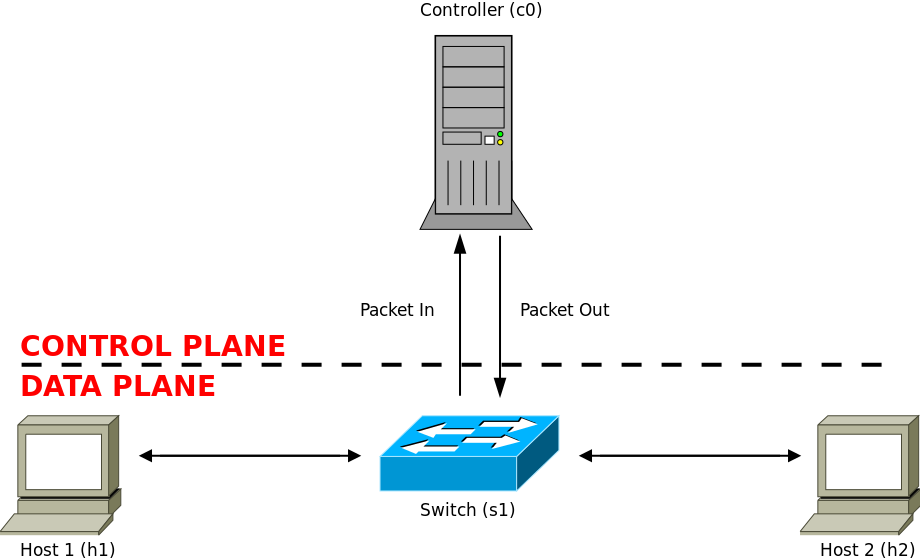
\includegraphics[width=\linewidth]{imagenes/Technologies/SDN.png}
  \caption{Sample SDN topology with a switch as forwarding device.}
  \label{fig:SDN_example}
\end{figure}

In practice, this method has many advantages. Here we list some of them.
\begin{itemize}
    \item \textbf{Cheaper hardware}. The networking devices become just forwarding devices, which do not need to have strong computational capabilities, and hence they can get rely on less powerful CPUs.
    \item \textbf{Global topology vision}. Having a centralized controller allows for a better vision and understanding of the entire network, making tasks such as traffic engineering far simpler.
    \item \textbf{Adaptability}. The controller can quickly reconfigure the forwarding devices if needed.
    \item \textbf{Scalability}. A controller can manage many forwarding devices (although it depends on the services implemented). However, it is possible to increase the number of controllers if necessary. 
    \item \textbf{Hardware agnostic}. Each physical device is just a generic forwarding device, all of the services and protocols are implemented via software on the controller.
\end{itemize}

In general, SDN are a great alternative to traditional networks. They are becoming more and more prevalent as time goes on, and rightfully so. For instance the up and coming 5G mobile technology will be based on this technology.

\section{OpenFlow}
Software Defined Networks and OpenFlow\cite{openflow_specfication} are tightly tied together, since OpenFlow is the communication protocol used between the forwarding devices and the controller or controllers. 

OpenFlow has two main messages, Packet\_In and Packet\_Out. The former, Packet\_In, is used to query the controller when the forwarding device does not know what to do with a certain packet or data stream. The latter, Packet\_Out, is the response to the Packet\_In message. It tells the forwarding device what to do with the packet and, optionally, it might install a flow on that device.

But, what is a flow? A flow is to a forwarding device what an entry in the routing table is to a traditional router. It basically tells the forwarding device what to do with a packet that matches certain fields. A flow has two major components:
\begin{itemize}
    \item \textbf{Matching fields}. As its name indicates, it contains the fields that a packet must match in order to follow this flow.   
    \item \textbf{Action}. What to do with the packet when it matches the flow.
\end{itemize}

A simple example is shown below. This example comes from the tool Open vSwitch, to which section \ref{section_ovswitch} offers a brief overview.
\begin{lstlisting}
    sudo ovs-ofctl add-flow s1 ip,nw_dst=10.0.0.1,actions=output:2
\end{lstlisting}

In this example, we are adding a new flow to a forwarding device called \textbf{s1}. In this flow we are specifying the matching fields as the IP protocol and the destination IP address \textbf{10.0.0.1}, while the action would be to output it through \textbf{port 2} of \textbf{s1}.

An OpenFlow flow supports a wide a variety of matching fields and actions, given the controller a high level of control and granularity over the forwarding devices.

It is also important to note that OpenFlow has several versions that, currently, go from 1.0 to 1.5, with each version mainly adding some new features. Due to technical reasons which will be later discussed, we will be using OpenFlow 1.0 for this project.

\section{Network Slicing Hypervisor}
This is the main element for the project. It is what allows us to slice a physical network into multiple virtual networks. A hypervisor sits between the OpenFlow switches and the controllers, redirecting each Packet\_In to its correspondent controller, as shown in Figure \ref{fig:hypervisor}. This way, a controller only sees a subset of the actual physical network, according to the packages received. Effectively, this is network slicing or virtualization.

If we dive more into the technical details, we find that what a hypervisor actually does, in its simplest form, is create flowspaces. A flowspace is nothing more but a rule or a set of rules that match the incoming packets and assign them to a particular slice.

\begin{figure}
  \centering
  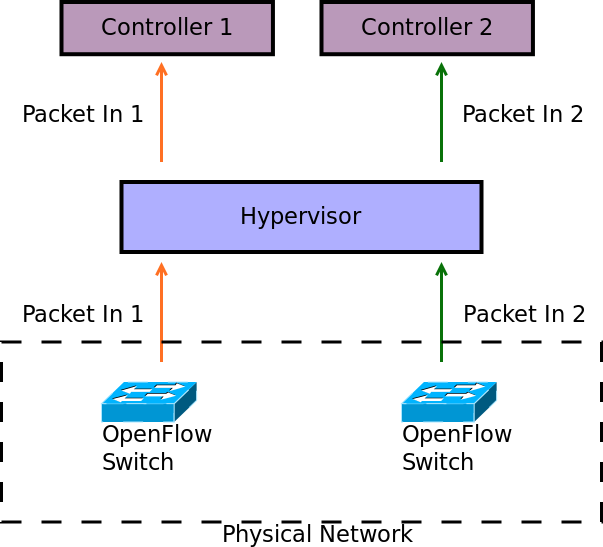
\includegraphics[width=\linewidth]{imagenes/Technologies/hypervisor.png}
  \caption{Simplistic overview of a network virtualization hypervisor.}
  \label{fig:hypervisor}
\end{figure}

In reality the way it works is very similar to just plain OpenFlow. There are rules that match certain packets but, instead of assigning an action to them, a slice is assigned. However, in this case only the Packet\_In are matched against the different rules, as opposed to every packet within the physical network.

Despite its potential usefulness, using a hypervisor also has a few downsides.
\begin{itemize}
    \item \textbf{Single point of failure.} A single hypervisor serves multiple controllers. As a result, a failure in the hypervisor may have extended consequences for several slices, effectively rendering the entire physical network, or a big part of it, unusable.
    
    \item \textbf{Added latency.} The introduction of an extra step for the packets results in a higher delay between the packet arrival and an action being taken. Said delay depends on several factors, e.g., the physical location of the hypervisor and the controllers. This extra delay may not be an issue for most applications, but it might affect the performance of real time applications with strict time constraints.
\end{itemize}

One could also argue that a hypervisor requiring extra configuration is also a downside. However, using a hypervisor usually helps simplify the logic of the controllers that sit above it, therefore reducing the time and cost needed to set up the network.

\section{Open vSwitch} \label{section_ovswitch}
Since we do not have access to physical OpenFlow switches, we have to rely on virtualization. Open vSwitch\cite{ovs_website} (OVS) is a tool that allows us to emulate one or multiple switches which support an ample amount of protocols, such as NetFlow, sFlow, IPFIX, RSPAN, CLI, LACP, 802.1ag, etcetera \cite{ovswitch}.

For the most part, we will not be using OVS directly as it is handled automatically by the the tool in section \ref{Mininet}, Mininet. However, OVS provides a useful command line interface that can prove very useful, especially for debugging, as it allows us to interact directly with the virtual switches. Some of these useful commands are shown below.

\begin{lstlisting}
# Shows the OpenFlow flows installed on a particular virtual switch.
sudo ovs-ofctl dump-flows <switch>
\end{lstlisting}

\begin{lstlisting}
# Useful to map the interface names to their corresponding 
# port number.
sudo ovs-ofctl show <switch>
\end{lstlisting}

\begin{lstlisting}
# Live update of the OpenFlow messages received by the virtual switch.
sudo ovs-ofctl snoop <switch>
\end{lstlisting}

\section{Mininet} \label{Mininet}
On the same topic of virtualization, we may come to the conclusion that virtual switches are not enough to emulate a network. This is the reason why we will use Mininet\cite{mininet_website}, an open source network emulator. While it is possible to do the network emulation manually without the help of Mininet, it would be immensely cumbersome, and thus we opt to use it for its convenience. 

Also, Mininet provides a powerful and easy to use Python API. With this API we can customize the network to our liking, allowing us to control a multitude of variables such as the bandwidth and delay between links, number of hosts, number of switches, number of links between each device, IP addresses, physical addresses and many more.

The power of Mininet resides within some useful features of the Linux kernel such as process groups, CPU bandwidth isolation and network namespaces. These features allow Mininet to produce a lightweight emulation of a small-to-medium size network within a single Linux kernel. In consequence, this is also a limitation, not allowing the hosts to be based on Windows, BSD or any other operating system \cite{mininet}.

Additionally, as we mentioned in section \ref{section_ovswitch}, by default Mininet makes use of Open vSwitch to virtualize the switches. This means that we can take advantage of the Open vSwitch command line interface for debugging and testing purposes.

Although Mininet offers a good amount of features, it does not implement an OpenFlow controller beyond its basic reference controller, meaning we have to implement it ourselves. Thankfully there are several libraries to ease this task like POX (Python) or Beacon (Java), so that it does not become an obstacle when deploying the network.

Lastly, as an example, Figure \ref{fig:mininet_default} shows the default topology created by Mininet, which is two hosts (h1 and h2) connected to one switch (s1) which in turn is connected to the reference controller (c0). The reference controller, albeit very basic, can manage ICMP traffic between the two hosts. This topology happens to be the same as the one shown in Figure \ref{fig:SDN_example}.

\begin{figure}
  \centering
  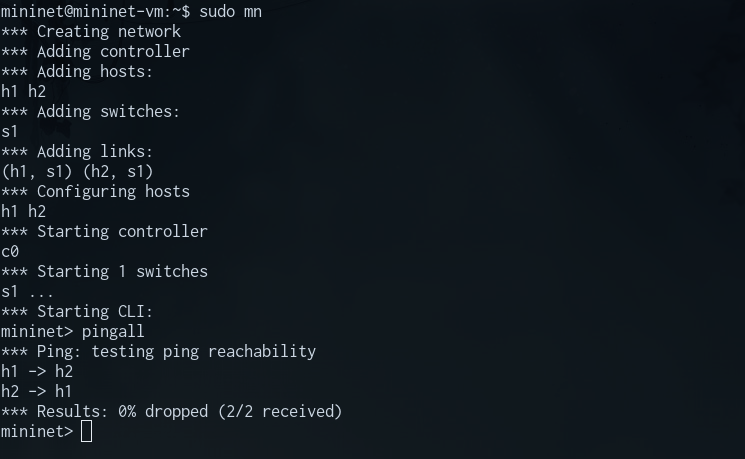
\includegraphics[width=\linewidth]{imagenes/Technologies/mininet_default_topology.png}
  \caption{Default Mininet topology.}
  \label{fig:mininet_default}
\end{figure}

\section{MQTT}
MQTT\cite{mqtt_specfication} was invented in 1999 by Dr Andy Stanford-Clark and can be defined as subscription based connectivity protocol. One of its main strengths is the small bandwidth requirement, it is a very lightweight protocol. Consequently, it makes for an ideal candidate for communications within the IoT environment.

Broadly speaking, the main idea behind MQTT consists on client A subscribing to one ore more topics. When a different client B publishes information under the same topic, it is forwarded to that client A as well as to every other client that is subscribed to that particular topic. In order for this system to work, a third element called \textbf{broker} is placed in between both clients, see Figure \ref{fig:mqtt}. The broker relays each published message to the correspondent subscribers of that topic.

Finally, MQTT spans over different versions, but versions 5.0 and 3.1.1 are of particular importance, as they are OASIS standards.

\begin{figure}
  \centering
  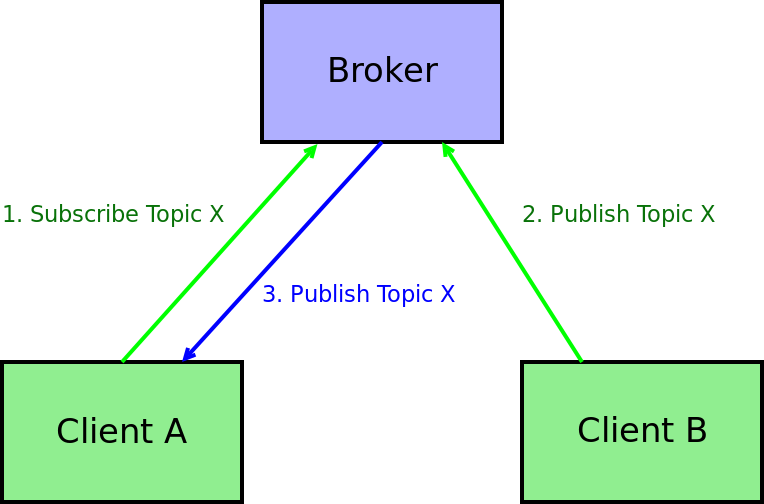
\includegraphics[width=\linewidth]{imagenes/Technologies/mqtt.png}
  \caption{Simplified example of a message transaction using MQTT.}
  \label{fig:mqtt}
\end{figure}

\section{LoRa}
LoRa\cite{lora_website}, currently being developed by Semtech, is a physical layer wireless communication protocol. It is quite a recent technology and it has been growing as a result of the current trend of the Internet of Things.

LoRa is quite a complex technology and it could have its own chapter. Nevertheless, here are, in a very over-simplified way, the main attributes of LoRa.
\begin{itemize}
    \item It relies on the unlicensed Industrial, Scientific and Medical (ISM) band. For example, Europe uses the \SI{868}{\mega\hertz} band while Asia and USA use \SI{433}{\mega\hertz} and \SI{915}{\mega\hertz} respectively. 
    \item Uses a spread spectrum technique based on chirp signals.
    \item Adaptable bandwidth with SNR trade off.
    \item Low power consumption.
    \item Long range communications, emphasized on rural areas. 
    \item Low cost and fairly straightforward to implement.
\end{itemize}

Due to its low power consumption and long range qualities, LoRa fits perfectly as the data communication protocol for IoT devices, especially in rural areas.

\subsection{LoRaWAN}
Tied to LoRa lies LoRaWAN\cite{lorawan}, a Wide Area Network specification based on LoRa. In a LoRaWAN network, there are typically four key components, see Figure \ref{fig:lorawan}.
\begin{itemize}
    \item \textbf{LoRa endpoints}, e.g., sensors. They send data to the network wirelessly through LoRa.
    \item \textbf{Gateway}. Receives the data from the sensors and forwards it, via conventional means (WiFi/Ethernet/Cell network), to the network server.
    \item \textbf{Network server}. Performs some authentication checks and traffic management operations. Eventually sends the data to the application.
    \item \textbf{Application}. Receives the data originally sent by the LoRa endpoint and forwards it to the client that requested it. Typically, this data forwarding is done using MQTT or a REST API.
\end{itemize}

Additionally, LoRaWAN also takes care of Media Access Control (MAC) as well as network security, e.g., authentication and integrity.

\begin{figure}
  \centering
  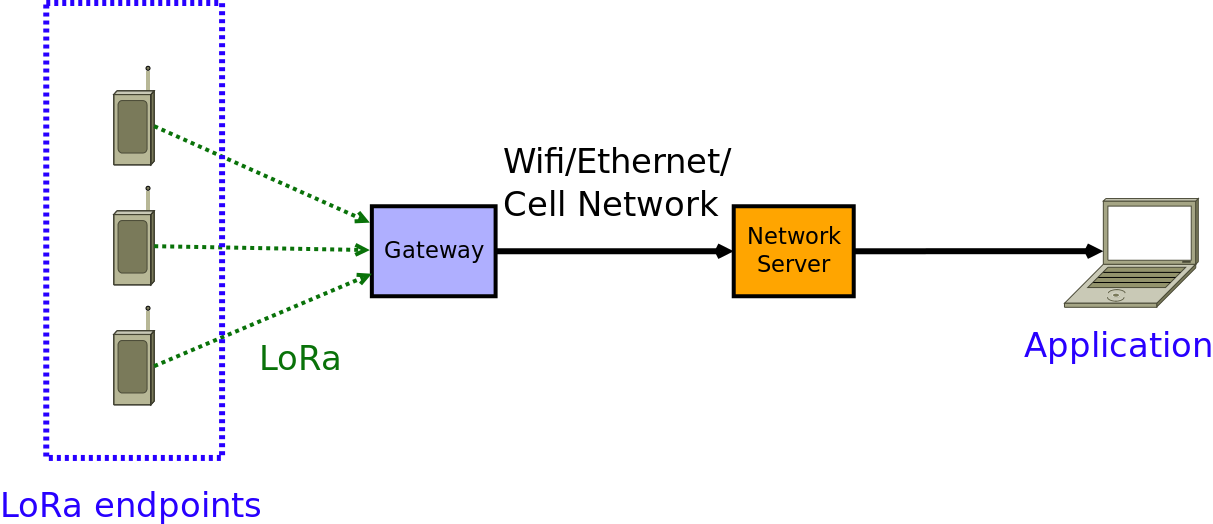
\includegraphics[width=\linewidth]{imagenes/Technologies/lorawan.png}
  \caption{LoRaWAN example network.}
  \label{fig:lorawan}
\end{figure}

\chapter{State of the Art} \label{chapter:state_of_the_art}
There are several hypervisors that have been developed in the last few years, as well as SDN controllers. We will now consider the benefits and drawbacks of each alternative and, at the end of the chapter, explain the rationale behind the ones we will end up using. 

Regarding the hypervisors, some, if not most, of them are not really usable in the present day, i.e., they are only a prototype or a proof of concept. They will be mentioned regardless for the sake of completeness.

\section{Hypervisor Candidates}
For each entry, we will avoid the implementation and technical details. The point of this section is to offer a fairly simple overview for each hypervisor, with just enough details so that we can make a decision on whether to use it or not.

\subsection{CoVisor}
CoVisor is defined as "A new kind of network hypervisor that enables, in a single network, the deployment of multiple control applications written in different programming languages and operating on different controller platforms"\cite{covisor}.

CoVisor's main selling point is its flexibility, it is intended to allow different technologies to work together in order to create a "best of breed" network, as its authors call it. They also have a strong consideration for efficiency, as they mention how to exploit new efficient algorithms.

While CoVisor seems like a valid choice, it presents two problems for this project in particular.
\begin{itemize}
    \item Adds unnecessary complexity. We are looking for a simple hypervisor that will allow us to slice a network. CoVisor does this, but it is designed for handling many different controllers at once, which gets very complex very fast.
    \item It is nothing more than a proof of concept. There is no code available that we can use to test it, at least not at the time of writing this document.
\end{itemize}

\subsection{FlowVisor}
Flowvisor is a hypervisor developed at Standford University. It is also fairly simple. It creates different slices which correspond to different controllers and relays the packets accordingly. Flowvisor is also open source and there are some good examples about network slicing available online.

Flowvisor looks like a good candidate for the project, but it has a few drawbacks.
\begin{itemize}
    \item Despite being open source, it has not been updated since 2013.
    \item It only works with OpenFlow 1.0.
    \item It definitely lacks some proper documentation about its features and implementation details.
    \item The slices are restricted to a subset of the physical topology.
\end{itemize}

The fact that FlowVisor has not been updated in years and the lack of documentation seem to be linked, as the code itself seems to work for the most part. It looks like FlowVisor is just lacking a cleaner API due to the absence of updates, aside from the OpenFlow version compatibility issue.

Regardless of these issues, FlowVisor is very widespread and is commonly used, probably due to the fact that is open source. This ensures that it has been tested thoroughly in many different topologies, thus improving its stability and minimizing possible bugs.

\subsection{VeRTIGO}
VeRTIGO stands for ViRtual TopologIes Generalization in Openflow networks \cite{vertigo}. It is presented as an extension to FlowVisor, aiming to overcome its limitations. One of these limitations, as mentioned by the authors of VeRTIGO, is the fact that the virtual topologies created by FlowVisor are just a subset of the physical topology.

The authors' idea is based on enhancing FlowVisor's "intelligence" in order to circumvent its limitations in slice creation and management, as well as increasing its robustness to network congestion and link failures. They also mention to have performed some testing in a real production environment.

Since VeRTIGO is presented as an extension to FlowVisor, it looks like a good choice. However, it seems like VeRTIGO never made it out of the prototype phase and it is not available for public use.

 \subsection{RadioVisor}
 As its name indicates, RadioVisor\cite{radiovisor} is a hypervisor designed around Radio Access Networks. The authors point out the current difficulties and cost of deploying basetations. They mention SoftRAN\cite{softran}, which is SDN technology applied to Radio Access Network, as an improvement over the situation. However, they argue that a better solution would be to extend SoftRAN and use RadioVisor to dynamically slice the network based on traffic and congestion. Unlike conventional hypervisors, RadioVisor also has to take into account the possible interferences between the different slices. Now, there are a few issues with this hypervisor.
\begin{itemize}
    \item Too specialized. We are looking for a more general purpose hypervisor that supports a broader array of networks.
    \item As with many other hypervisors in this chapter, we have been unable to find the source code or a functional version of it.
\end{itemize}

\subsection{AutoSlice}
AutoSlice\cite{autoslice} is slightly different from the rest of the hypervisors discussed in this chapter. It not only aims to provide slicing capabilities, its main goal is to automate such process. By relaying on automation, it would be possible to rent an SDN to different tenants while minimizing the need for manual intervention. This is made possible by giving each tenant the means to lease "programmable network slices", according to the authors. An overview of this architecture is shown in Figure \ref{fig:autoslice}.

\begin{figure}
  \centering
  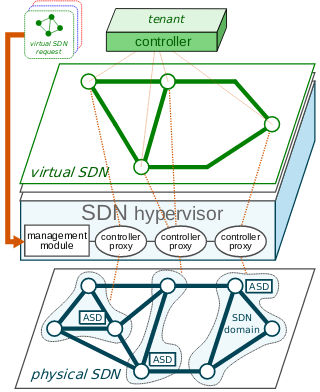
\includegraphics[width=0.6\linewidth]{imagenes/StateOfTheArt/AutoSlice_architecture.png}
  \caption[AutoSlice architecture.]{AutoSlice architecture\cite{autoslice}.}
  \label{fig:autoslice}
\end{figure}

One issue that arises when reading the article about AutoSlice, is that it has only been tested with OpenFlow 1.0. Ideally we would like to use a hypervisor that is capable of handling the latest version of OpenFlow, i.e, OpenFlow 1.5.

Regarding the viability of this hypervisor, it is too complex for what we are trying to do. But even if we wanted to use it, there is no code in sight. It seems like it was just a proof of concept. 

\subsection{ADVisor}
The authors of ADVisor\cite{advisor} refer to FlowVisor as a recent approach towards network virtualization. However, they also acknowledge its limitations when it comes to flowspace sharing and traffic interferences. They propose ADVisor (ADvanced Flowvisor) as a way to overcome those limitations. 

ADVisor is designed to extend FlowVisor in order to provide two additional virtualization functions: Virtual link management, and Virtual ports management. As a result, ADVisor is able to work with FlowVisor in a nested way, as shown in Figure \ref{fig:advisor}.

\begin{figure}
  \centering
  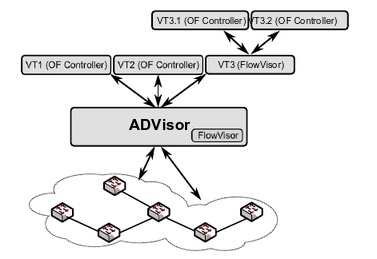
\includegraphics[width=0.8\linewidth]{imagenes/StateOfTheArt/ADvisor_architecture.png}
  \caption[ADVisor architecture.]{ADVisor architecture\cite{advisor}.}
  \label{fig:advisor}
\end{figure}

As for the possible drawbacks, ADVisor seems to slightly surpass the scope of this project. And, again, it appears to be just a proof of concept with no source code or binary files available for us to test it.

\section{OpenFlow Controllers}
This section will go through a quick overview of the most popular OpenFlow controllers, hoping to find the most suitable one for the project.

\subsection{NOX}
NOX was the first OpenFlow controller. Originally developed by Nicira Networks and then released to the research community back in 2008. According to its archived website\cite{nox}, NOX had the following features: 
\begin{itemize}
    \item C++ OpenFlow 1.0 API.
    \item Fast, asynchronous IO.
    \item Targeted at Ubuntu 11.10 and 12.04.
    \item Includes sample components: Topology discovery, learning switch and network-wide switch.
\end{itemize}

It is evident that NOX is heavily outdated and its use is not recommended. Nonetheless, it is featured in this chapter as it is the predecessor to another popular SDN controller, POX.

\subsection{POX}
While the last time POX was updated was two years ago, it is still much more recent than NOX. Although POX is considered the successor to NOX, POX's features differ considerably from NOX's.
\begin{itemize}
    \item Python 2.7 OpenFlow API.
    \item Supports pretty much anything that can run Python 2.7 (Windows, Mac OS, Linux, Android, FreeBSD, etc).
    \item Support for PyPy JIT compiler for a performance boost.
    \item It can only handle OpenFlow 1.0.
    \item Includes a wide variety of sample components.
\end{itemize}

Moreover, POX comes already bundled with the Mininet virtual machine, so it does not require any additional installation. 

\subsection{OpenDaylight Controller}
Founded in 2013, the OpenDaylight foundation develops a very popular open source SDN controller platform. They are also a member of the Linux Foundation Networking. They like to name each release after an element from the periodic table, the most recent one being Neon, which is their tenth release (Neon's atomic number is 10). OpenDaylight Neon is the most complex SDN controller featured in this section. For an overview of its architecture, see Figure \ref{fig:opendaylight}.

\begin{figure}
  \centering
  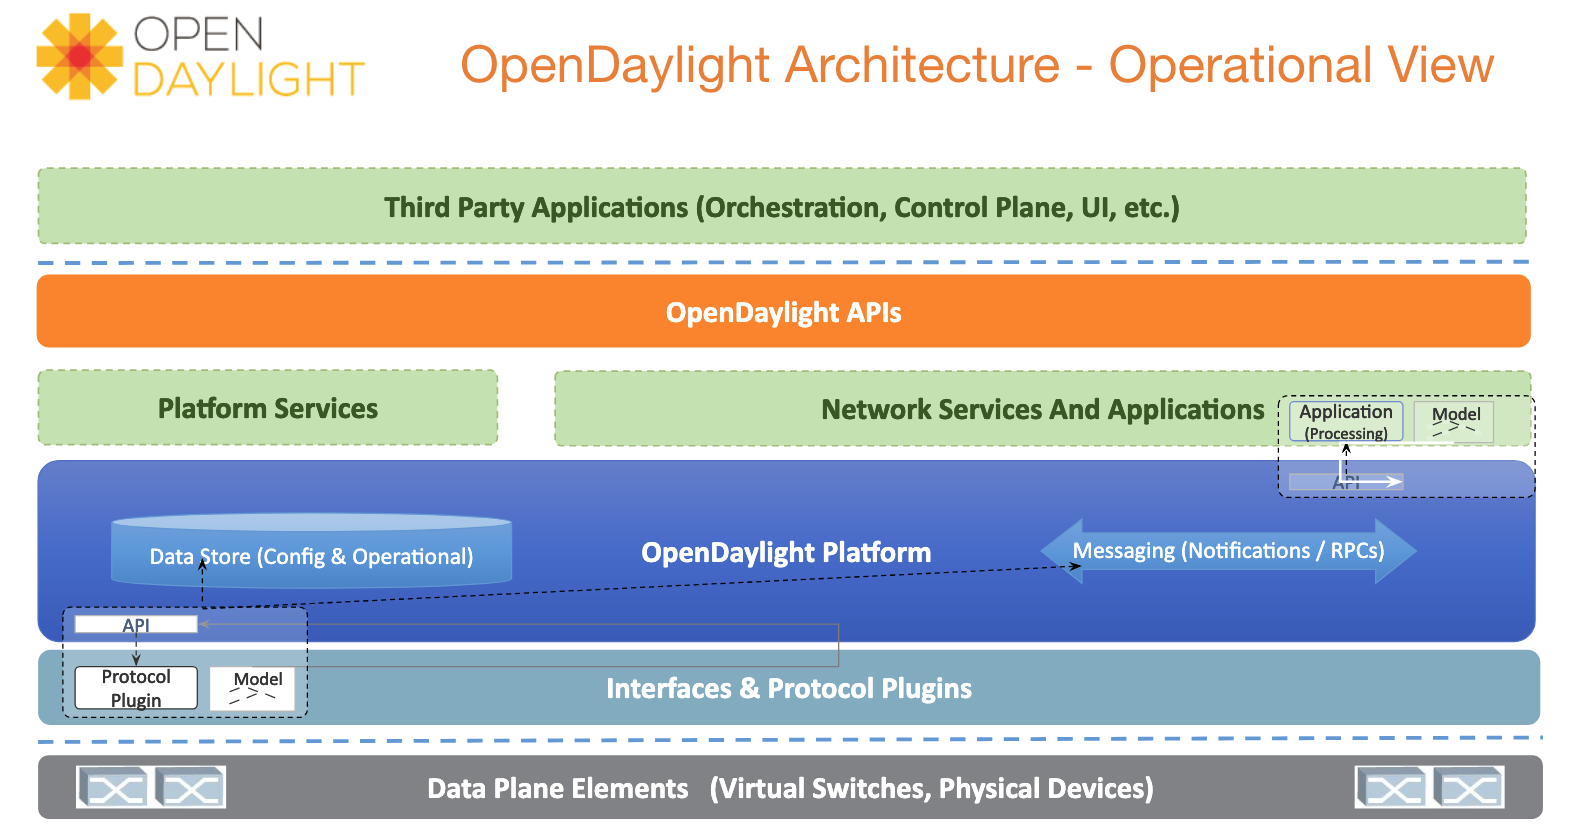
\includegraphics[width=0.8\linewidth]{imagenes/StateOfTheArt/open_daylight.png}
  \caption[OpenDaylight Neon architecture overview.]{OpenDaylight Neon architecture overview\cite{opendaylight}.}
  \label{fig:opendaylight}
\end{figure}

OpenDaylight main advantages are:
\begin{itemize}
    \item Thoroughly tested and production ready. Used by a lot of companies all over the world.
    \item Supported by big companies such as AT\&T, Cisco and Ericsson among others.
    \item Plenty of features from more than 100.000 commits, e.g, cloud network virtualization.
    \item Modular. Only install features you need.
    \item Graphical interface. Makes it more user friendly than terminal-only controllers.
    \item Good documentation.
\end{itemize}

OpenDaylight is a great controller. However, and despite being modular, it is quite heavier memory wise than the rest of alternatives. It is also written in Java, so a JRE is needed in order to run the OpenDaylight controller. 

\subsection{Beacon}
Developed at the Standford University in 2010, Beacon\cite{beacon} is an open source OpenFlow controller written in Java. Beacon was mostly designed with three goals in mind.
\begin{itemize}
    \item Developer Productivity.
    \item Runtime Modularity. The goal is to be able to start and stop applications while the controller itself is running.
    \item Performance. Multi thread implementation.
\end{itemize}

Beacon, like NOX, is quite outdated with its last update happening on May of 2011. Nevertheless, Beacon is an OpenFlow controller worth mentioning, as it is the base for another controller, Floodlight.

\subsection{Floodlight}
Floodlight started as fork of Beacon in 2011, therefore it is also open source. Unlike Beacon, Floodlight's last update, at the time of writing this document, was released on May of 2019. Floodlight's main strengths are:
\begin{itemize}
    \item Well tested.
    \item Good documentation.
    \item Includes sample components.
    \item Graphical interface.
    \item Supports OpenFlow from version 1.0 to 1.5.
    \item Modular.
    \item Multi threaded. 
    \item Can handle mix-OpenFlow and non OpenFlow networks.
\end{itemize}

In addition, despite Floodlight being written in Java, it can be extended using its REST API. In fact, its sample components use Python to access the REST API.

\section{Conclusions}
It is now time to make a decision and choose from the several options presented in this chapter. In regards to the OpenFlow controller, we could choose more than one since we intend to use multiple controllers. Because of the added complexity that using different controllers entails, we will just choose one. 

\subsection{Hypervisor}
Given that only one of the previous entries is a valid candidate, i.e., it is publicly available, it is trivial to make the choice, we will use FlowVisor. It has a few inconveniences, e.g., lack of proper documentation and limited version compatibility with OpenFlow. Nonetheless, FlowVisor should be sufficient to carry out the project.

There are some more hypervisors that have not been mentioned, yet none of them are publicly available at the time of writing this document.

It seems like the developing of hypervisors for network slicing/virtualization was a hot topic a few years ago, but either almost none of them made it past the proof of concept or they were completely privatized and used internally within the industry. Furthermore, the only one that made it to open source, i.e., FlowVisor, was pretty much abandoned for unknown reasons as its three contributors moved on to different projects.

\subsection{OpenFlow Controller}
The OpenFlow controller section is much more competitive than the hypervisor section. There are multiple good choices, each one with its pros and cons. In order to make the best decision, let us establish the baselines for what we want from a controller.
\begin{itemize}
    \item Simple and lightweight. The whole point of using a hypervisor is to simplify the logic of the controller.
    \item Python based. This is mainly a preference, as Python is the language we are most proficient at.
    \item No need to support OpenFlow higher than 1.0, since FlowVisor itself only supports OpenFlow 1.0.
    \item High performance is not a concern. The logic of the controller will be very simple.
    \item Well documented or includes sample components.
    \item A graphical interface is not necessary.
    \item Not extremely outdated.
\end{itemize}

Given these requirements, the controller that fits the most is the POX controller. POX is simple enough for what we need, lightweight, comes with sample modules, extendable with Python and, on top of that, it comes already installed with the Mininet Virtual Machine.

\chapter{Time Management and Cost Estimate}
We now briefly describe the multiple stages of this project, along with their corespondent time constraints and associated cost. By the end of this chapter, we will have a rough idea of the total time needed to carry out the project as well as an estimate for its total monetary cost.

The chapter will be broken down into two main sections. The first one will focus on the time aspect of the project, while the second one will address the cost.

In regard to estimating the cost, it will be broken down into two groups.
\begin{itemize}
    \item \textbf{Human resources}. Very rough estimate of the amount of work hours needed for each person involved, along with the total cost when computing in the value for each hour and for each person.
    \item \textbf{Hardware and software}. Cost of the equipment needed as well as any non-free software used.
\end{itemize}

\section{Time Management}
In this section, we will attempt to calculate how long will this project take. Afterwards, a Gantt chart, Figure \ref{fig:gantt_chart}, visualizes the time cost for each development stage. For the begin and end date of each stage, refer to Table \ref{tab:gantt_dates}.

Moreover, this estimation is done prior to starting the project. It may or may not correspond to the actual amount time the project required. The main goal of this section is to have a point of reference we can fall back during the realization of the project.

With that in mind, here we enumerate every development stage with a significant time cost.
\begin{itemize}
    \item \textbf{State of the Art revision}. A study of the already existing solutions is necessary in order to choose the most suitable one.
    \item \textbf{Testing Environment Setup}. Since we lack a physical network for testing, we need to set up a robust virtual environment. 
    \item \textbf{Implementation}. Once the testing environment is ready, we can begin to configure FlowVisor.
    \item \textbf{Testing}. We make sure the hypervisor works as expected and the configuration is correct.
    \item \textbf{Documentation}. This is technically not a stage, as it spans the entire duration of the project. It is also not tied to any other stage in particular, so it can be done in parallel.
\end{itemize}

\begin{figure}
  \centering
  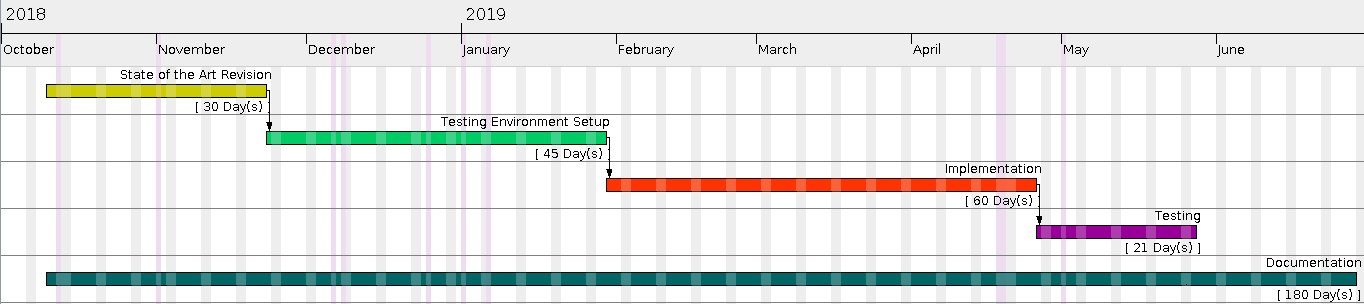
\includegraphics[width=\linewidth]{imagenes/TimeCost/Gantt_chart.png}
  \caption{Gantt Chart.}
  \label{fig:gantt_chart}
\end{figure}

\begin{table}
    \centering
    \caption{Duration, begin date and end date for each development stage.}
    \vspace{0.1 cm}
    \begin{tabular}{l c c c}
    \hline
    \rowcolor{lightgray}
    \textbf{Development stage}           &\textbf{Duration} &\textbf{Start}   &\textbf{End}            \\ \hline
    State of the art revision            & 25 days          & 10/10/2018      & 22/11/2018             \\ \hline 
    Environment Setup                    & 45 days          & 23/11/2018      & 29/01/2019             \\ \hline
    Implementation			             & 60 days          & 30/01/2019      & 25/04/2019             \\ \hline
    Testing          		             & 21 days          & 26/04/2019      & 27/05/2019             \\ \hline
    Documentation			             & 183 days         & 10/10/2018      & 28/06/2019             \\ \hline
    \end{tabular}
    \label{tab:gantt_dates}
\end{table}

From this data, we estimate this project's length to span over 183 days. This is the duration of the documentation stage, as we consider it to be the bottleneck.

\section{Cost Estimate}
This section will cover the estimation of the budget necessary to carry out the present project. Moreover, it is not the intent of this section to provide a very accurate answer. On the contrary, the actual purpose is just to obtain an approximate cost that would be within the same order of magnitude of the actual cost if it were possible to compute.

Furthermore, to make the estimate geographically agnostic, prices will not include VAT nor shipping cost when applicable.

\subsection{Human Resources}
The following people have worked or contributed to this project in one way or another:
\begin{itemize}
    \item \textbf{Jorge Navarro-Ortiz}. Associate professor of the Department of Signal Theory, Telematics and Communications of the University of Granada, as thesis supervisor.
    \item \textbf{Angel Guzman-Martinez}. Student of the School of Informatics and Telecommunications Engineering of the University of Granada.
\end{itemize}

Currently in Spain, disclosing a salary/price of reference for any profession or service is forbidden by law \cite{spanish_government_defensa_2007}. Therefore, this category will be based on the assumption that a telecommunication engineer, usually earns no less than \EUR{20} per hour and no more than \EUR{50} per hour. From there, we have decided to assign \EUR{25}/h to Angel Guzman-Martinez and \EUR{50}/h to Jorge Navarro-Ortiz.

In order to compute the actual cost for each person, we also need to estimate the amount of hours contributed towards the project. Again, this will be just an approximation.

\begin{itemize}
\item Angel Guzman-Martinez: 3 hours a day during 9 months excluding weekends. This yields, approximately, \textbf{594 hours.}
\item Jorge Navarro-Ortiz: \textbf{8 hours} in total of tutorship.
\end{itemize}

Taking everything into account, the total cost for human resources amounts to \textbf{\EUR{15,250}}. Refer to Table \ref{tab:HumanResources} for a quick summary.

\begin{table}
    \centering
    \caption{Human resources cost.}
    \vspace{0.1 cm}
    \begin{tabular}{l c c c}
    \hline
    \rowcolor{lightgray} \textbf{Concept}&\textbf{Cost/time}&\textbf{Quantity}&\textbf{Total}          \\ \hline
    Project work		  	             & \EUR{25}/h       & 594 hours       & \EUR{14,850}           \\ \hline 
    Tutorship				             & \EUR{50}/h       & 8 hours         & \EUR{400}              \\ \hline
    \textbf{Total}				         &                  &                 & \textbf{\EUR{15,250}}  \\ \hline 
    \end{tabular}
    \label{tab:HumanResources}
\end{table}

\subsection{Mandatory Hardware and Software}
It is important to note that, in this section, we will only list the hardware and software strictly necessary for the project to work. Whatever was used exclusively for the testing phase will be addressed later in this chapter. With that said, here is the list of critical components:

\begin{itemize}
    \item \textbf{Laptop.} The physical platform that will host the Mininet virtual machine. Any laptop that is able to run virtualization software will do. In our case we use HP 250 G6 Notebook with an Intel i5-7200U CPU, an Intel HD Graphics 620 integrated GPU and 8GB of RAM.
    
    \item \textbf{GNU/Linux}. Our operative system of choice and it is free. In particular, we use the Arch Linux distribution with the Linux kernel version 5.1.3. There are many others free  distributions, as well as a paid alternative, i.e., Windows. Any of them would work just fine as long as they are able to run some kind of operative system virtualization.
    
    \item \textbf{Virtual Box.} Software used for operative system virtualization. Virtualbox is what we used for this project in order to deploy the Mininet virtual machine, but there are a few alternatives, e.g., QEMU or VMware. 
    
    We could also use Mininet natively if we already have a GNU/Linux installation, yet it is still beneficial to use the standalone virtual machine as it provides a custom kernel optimized towards network virtualization.
    
    \item \textbf{Mininet.} Framework that allows us to create a virtual network within a single device. Ideally, in an real scenario, a physical network would be used. However, we did not have that possibility, so the budget estimate will be based on what we have actually used.
    
    \item \textbf{FlowVisor.} Open source SDN hypervisor used for network slicing.
\end{itemize}

Thankfully, all of the software we need is open source and free for personal use, see Table \ref{tab:software}. In the case of Virtual Box, a license is required for commercial use, which is not our case.

As for the hardware, see \ref{tab:hardware}.

\begin{table}
    \centering
    \caption{Mandatory Hardware cost.}
    \vspace{0.1 cm}
    \begin{tabular}{l c c c c c}
    \hline
    \rowcolor{lightgray}
    \textbf{Concept}&\textbf{Unit cost}&\textbf{Units} &\textbf{Average lifespan}&\textbf{Time used} &\textbf{Total}     \\ \hline
    Laptop          & \EUR{700}        & 1             & 3 years                 & 183 days          &\EUR{117}          \\ \hline
    \textbf{Total}  &                  &               &                         &                   &\textbf{\EUR{117}} \\ \hline 
    \end{tabular}
    \label{tab:hardware}
\end{table}

\begin{table}
    \centering
    \caption{Mandatory Software cost.}
    \vspace{0.1 cm}
    \begin{tabular}{l c c c}
    \hline
    \rowcolor{lightgray}
    \textbf{Software}&\textbf{Open source}&\textbf{Free for personal use} &\textbf{License cost}             \\ \hline
    Virtual Box      & Yes                & Yes    			  	          &\EUR{0}                           \\ \hline 
    Mininet          & Yes                & Yes    			  	          &\EUR{0}                           \\ \hline 
    FlowVisor        & Yes                & Yes    			  	          &\EUR{0}                           \\ \hline 
    \textbf{Total}   &                    &                          	  &\textbf{\EUR{0}}                  \\ \hline 
    \end{tabular}
    \label{tab:software}
\end{table}

\subsection{Hardware and Software Used for Testing}
This section is included for completeness, and it will list everything that was used exclusively for testing. It is worth noting that there are plenty of alternatives as to how we have performed the testing, so that it is not necessary to use the same elements that are shown here.
\begin{itemize}
    \item \textbf{Raspberry Pi}. Used as external physical host. To be more specific, we will use a model 3B running the Raspbian operative system and kernel Linux 4.9.69-v7+. 
    
    \item \textbf{LoRa mote}. It will be tasked to periodically send LoRa packets. The exact model is TTGO LoRa32 V2.1\_1.6.
    
    \item \textbf{LoRa gateway}. Its purpose is to receive the LoRa packets and forward them through our Mininet network and towards a physical external host. The model we will use is called LoRa Lite Gateway, developed by IMST.
\end{itemize}

Note how there is no specific software used exclusively for testing, so everything will be summarized in Table \ref{tab:testing_hardware}.

\begin{table}
    \centering
    \caption{Testing Hardware cost.}
    \vspace{0.1 cm}
    \begin{tabular}{l c c c}
    \hline
    \rowcolor{lightgray}
    \textbf{Concept}&\textbf{Unit cost}&\textbf{Units}              &\textbf{Total}         \\ \hline
    Raspberry Pi    &\EUR{33.94}       & 1 	                        &\EUR{33.94}            \\ \hline 
    LoRa mote       &\EUR{18.84}       & 1 	                        &\EUR{18.84}            \\ \hline 
    LoRa gateway    &\EUR{199}         & 1 	                        &\EUR{199}              \\ \hline 
    \textbf{Total}  &                  &                            &\textbf{\EUR{251.78}}  \\ \hline 
    \end{tabular}
    \label{tab:testing_hardware}
\end{table}

\subsection{Total Cost}
Lastly, we present two different budget estimates.
\begin{itemize}
    \item \textbf{Only mandatory components}. A cheaper alternative that dismisses anything that is not strictly necessary for the project to work, Table \ref{tab:mandatory_budget}.
    \item \textbf{Complete budget}. Includes the mandatory components as well as the hardware and software that was used exclusively for testing, Table \ref{tab:complete_budget}.
\end{itemize}

\begin{table}[H]
    \centering
    \caption{Mandatory budget.}
    \vspace{0.1 cm}
    \begin{tabular}{l c c c}
    \hline
    \rowcolor{lightgray} \textbf{Concept}  &\textbf{Cost}               \\ \hline
    Human resources                        &\EUR{15,250}                \\ \hline 
    Hardware						       &\EUR{117}                   \\ \hline 	
    Software                               &\EUR{0}                     \\ \hline
    \textbf{Total}                         &\textbf{\EUR{15,367}}       \\ \hline   
    \end{tabular}
    \label{tab:mandatory_budget}
\end{table}

\begin{table}[H]
    \centering
    \caption{Complete budget.}
    \vspace{0.1 cm}
    \begin{tabular}{l c c c}
    \hline
    \rowcolor{lightgray} \textbf{Concept}  &\textbf{Cost}               \\ \hline
    Human resources                        &\EUR{15,250}                \\ \hline 
    Mandatory Hardware					   &\EUR{117}                   \\ \hline 	
    Testing Hardware					   &\EUR{251.78}                \\ \hline 	
    Software                               &\EUR{0}                     \\ \hline
    \textbf{Total}                         &\textbf{\EUR{15,618.78}}    \\ \hline   
    \end{tabular}
    \label{tab:complete_budget}
\end{table}

If we only take into account the mandatory assets, this project will need, approximately, a budget of \textbf{\EUR{15,367}}. 

\bigskip

On the other hand, if we include everything then we have an approximate cost of \textbf{\EUR{15,618.78}}.
\chapter{Environment Setup} \label{chapter:environment}
As we have mentioned before, ideally the project's environment would be a physical network with OpenFlow switches. Since that is not possible for us, we will set up a virtual environment using a Mininet virtual machine. Consequently, this chapter will walk us through the process of setting up the virtual machine as well as the creating the network topology.

\section{Mininet Virtual Machine}
As a reminder, a virtual machine is not strictly necessary, as it can be installed natively in an already existing GNU/Linux system. Nonetheless, virtualization has a few advantages:
\begin{itemize}
    \item \textbf{Custom Linux kernel}. The Mininet virtual machine includes a custom Linux kernel optimized towards network virtualization.
    \item \textbf{Isolation}. It allows us to work on an isolated environment, so that the host system does not interfere. In essence, we have a simplified system that is easier to troubleshoot in the event that something goes wrong.
    \item \textbf{Repeatability}. We can reproduce the environment in different machine without having to reconfigure everything from scratch.
\end{itemize}

On the other hand, using a virtual machine also comes with some disadvantages such as extra overhead and networking becomes slightly trickier.

With that said, the very first thing we need to do is download the image file, which can be found here \url{https://github.com/mininet/mininet/wiki/Mininet-VM-Images}. There are several images to choose from, although most of them are deprecated old versions. Since we are running GNU/Linux as the host system, we have chosen "Mininet 2.2.2 on Ubuntu 14.04 LTS - 64 bit", which is the latest version at the time of writing this document.

Next up, after the download and decompressing the file, we are left with two files with the extensions ".ovf" and ".vmdk". The easiest way to proceed is to import the image using the ".ovf" file. If, for some reason, the import fails, we can manually create a new virtual machine and use the ".vmdk" file as hard disk.

After importing the image, we can now launch it and log in. The default credentials for username and password are mininet and mininet respectively. When we log in, we will notice that image does not include a display renderer, i.e., we do not have a graphical environment. From here we have three options.
\begin{enumerate}
    \item Work without a graphical environment and within the native Virtual Box terminal. The easiest option, does not require any extra configuration but it is also very limited and cumbersome. This option would not allow us to use graphical applications such as Wireshark.
    
    \item Install a display renderer and desktop environment or window manager. This requires quite a lot of extra memory usage within the virtual machine as well as overhead. In spite of having a worse performance, it is the most user friendly option.
    
    \item SSH into the virtual machine and work from the host machine using X forwarding. Very little overhead but it requires some configuration for it to work properly. This option is only possible if the host machine is running a Xorg server (display renderer).
\end{enumerate}

We will stick to option three since it is the one we feel the most comfortable and our host meets the requirements. In order to do it this way, we have to do the following.
\begin{enumerate}
    \item In the virtual machine, make sure at least one network adapter enabled either in host-only or bridge mode. For the latter, ensure the host is already connected to a network.
    
    \item Find out the IP address of the network adapter we just enabled. If there are several network adapters enabled, it is possible that the one we are interested on does not have an IP address assigned to it. If that is the case, use the \textit{dhclient} command manually.
    
    \item Connect to the virtual machine using the following command.
    \begin{lstlisting}
        ssh -Y mininet@<IP Address>
    \end{lstlisting}
    
    The -Y flag stands for trusted X forwarding. Regular X forwarding has a 20 minutes timeout and causes some issues when using Xterm within Mininet. Note that trusted X forwarding should not be used lightly and could have security implications.
    
    \item (Optional). Generate a private and public key pair on the host and transfer the public key to the virtual machine under \\ /home/mininet/.ssh/authorized\_keys. This will allow us to log into the machine without having to type the password every time.
\end{enumerate}

Finally, in preparation for the testing phase, we need to enable two additional network adapters on bridge mode. We will use these adapters to connect two external physical hosts to the Mininet network. After all of this, we are done configuring the virtual machine itself. We are ready to start setting up the Mininet topology.

\section{Mininet}
First off, we need to know what topology we want to create and then implement it in Mininet. For this, Mininet offers two different ways we can: through the CLI or using its Python\footnotemark API. While the CLI is easy to use, it has some limitations, so we will use the Python API instead. The main reason for using the API is that it is only the way to connect external interfaces to the Mininet network, which we will need to do for the testing phase. 

\footnotetext{The API uses Python version 2.7, although the Mininet contributors are slowly adding compatibility for Python 3.6.}

\subsection{Topology}
As it has been mentioned in a previous chapter, we want to avoid an overly complex topology. The goal is to just demonstrate the use of network slicing within an SDN. For that, we have chosen the topology shown in Figure \ref{fig:mininet_topology}\footnotemark. Based on that topology, the goal will be to create two network slices, one for the \SI[per-mode=symbol]{1}{\mega\bit\per\second} path and second slice for the \SI[per-mode=symbol]{10}{\mega\bit\per\second} path. 

\footnotetext{This topology is mainly based on the one shown here \url{https://github.com/onstutorial/onstutorial/wiki/Flowvisor-Exercise}.}

\begin{figure}
  \centering
  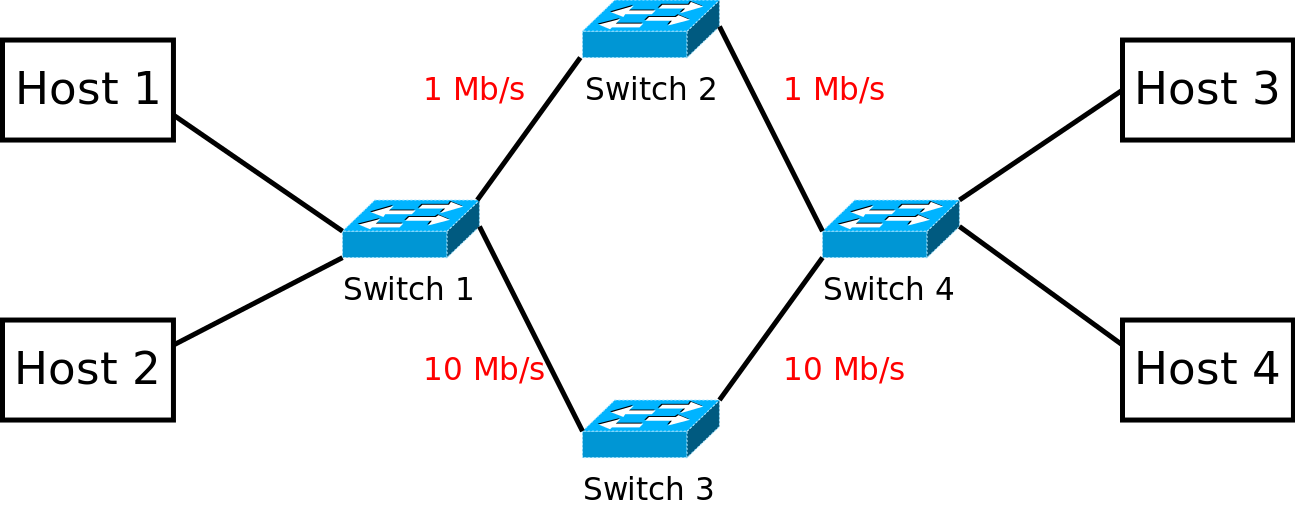
\includegraphics[width=\linewidth]{imagenes/Environment/mininet_topology.png}
  \caption{Base Mininet topology.}
  \label{fig:mininet_topology}
\end{figure}

Once we know what topology we want to create, we will use Mininet's Python API to build it. Alternatively, there is a GUI application called MiniEdit used to create a Mininet network in a visual way. Despite MiniEdit being the easier option, we will opt for the Python API because we would like to take a lower level approach. The code can be found at Appendix \ref{annex:mininet}.

To simplify the CLI command used to invoke the topology, we will place the Python file under /home/mininet/mininet/custom/.

Lastly, to build the network we use the command:
\begin{lstlisting}
    $ sudo mn --custom ~/onstutorial/flowvisor_scripts/<python filename> --topo <topology name> --link tc --controller remote --mac
\end{lstlisting}

Some of the flags used on the command above are not required to build our custom network, but they will be necessary for the testing process.
\begin{enumerate}
    \item \textbf{- -link tc}. Enables link bandwidth customization.
    \item \textbf{- -controller remote}. Will allow us to, later on, connect the network to FlowVisor.
    \item \textbf{- -mac}. (Optional). Disables MAC randomization for each host and makes it easier to associate each MAC to its correspondent host. This is very helpful for debugging.
\end{enumerate}

\subsection{Enabling External Hosts}
To prepare the topology for the coming tests, we have to adjust the network so that it can handle two external interfaces, Figure \ref{fig:mininet_topology_external}. This is where the Mininet CLI falls short. These external interfaces have to be added after the topology is created, which is not possible through the CLI. Therefore, we have to use the Python API for both creating the topology and running it.

\begin{figure}
  \centering
  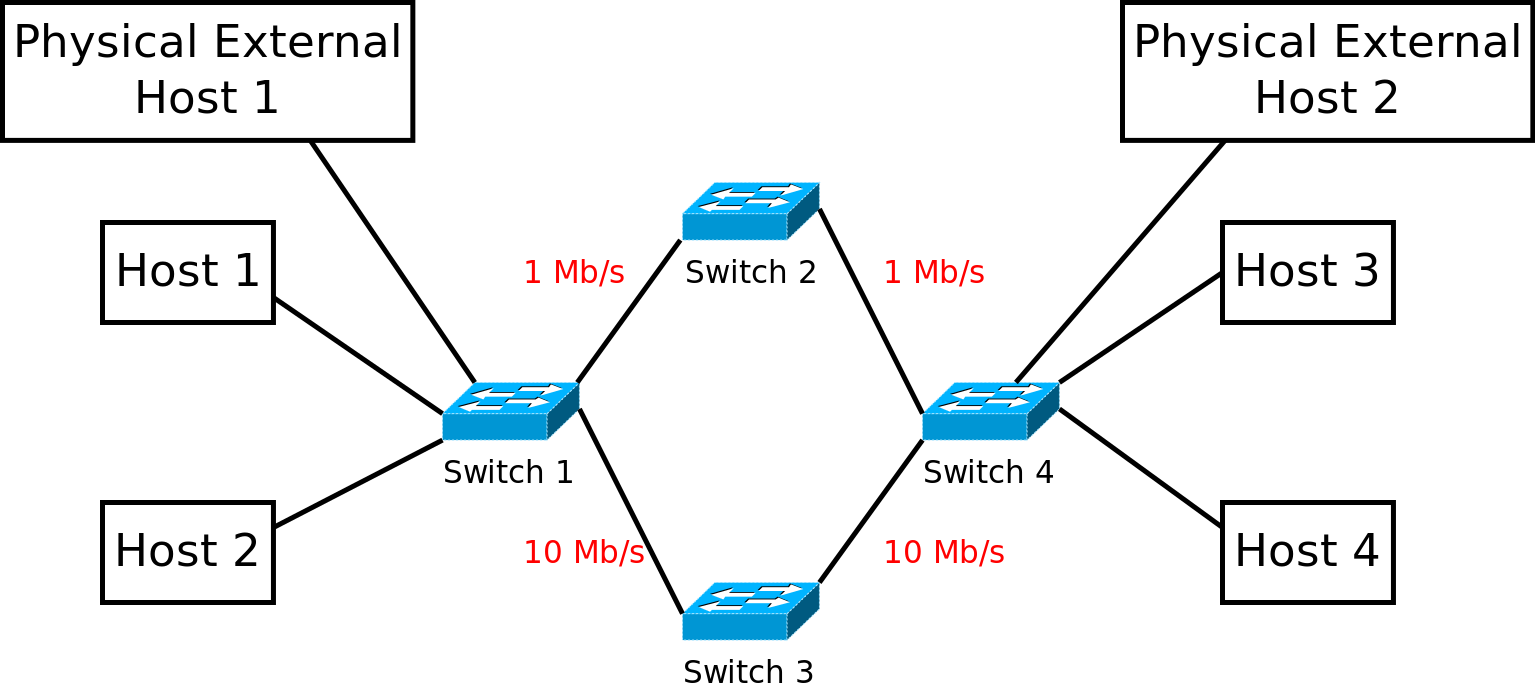
\includegraphics[width=\linewidth]{imagenes/Environment/mininet_topology_external_hosts.png}
  \caption{Mininet topology with added external hosts.}
  \label{fig:mininet_topology_external}
\end{figure}

Once the logic for running the network is added to the Python file, we no longer need to use the command line. We can launch the network by calling the Python file directly.
\begin{lstlisting}
    $ sudo python <python filename>
\end{lstlisting}

With the external interfaces added, our topology is almost ready to start handling some traffic. We are only lacking one element, although a very important one, a controller. An SDN becomes almost useless without a controller. However, an explanation on how to set up the controllers after can be found in the next chapter. 

\subsection{IP Address Assignment}
Finally, it is important to assign IP addresses correctly for the network to work correctly. We will not implement router functionality and as a result, hosts that want to communicate with each other must be assigned to the same sub network. IP assignments are shown in Tables \ref{tab:IP_virtual_hosts} and \ref{tab:IP_external_hosts} for virtual and physical hosts respectively. Since each host only has one available port, we will omit it.

\begin{table}
    \centering
    \caption{IP and MAC Addresses for the virtual hosts.}
    \vspace{0.1 cm}
    \begin{tabular}{c c c c}
    \hline
    \rowcolor{lightgray}
    \textbf{Virtual Host}               &\textbf{IPv4 Address} &\textbf{Network Mask}   &\textbf{MAC Address}     \\ \hline
    Host 1                              &  10.0.0.1            & 255.255.0.0            & 00:00:00:00:00:01       \\ \hline 
    Host 2                              &  192.168.0.2         & 255.255.0.0            & 00:00:00:00:00:02       \\ \hline 
    Host 3                              &  10.0.0.3            & 255.255.0.0            & 00:00:00:00:00:03       \\ \hline 
    Host 4                              &  192.168.0.4         & 255.255.0.0            & 00:00:00:00:00:04       \\ \hline 
    \end{tabular}
    \label{tab:IP_virtual_hosts}
\end{table}

\begin{table}
    \centering
    \caption{IP and MAC addresses for the physical hosts.}
    \vspace{0.1 cm}
    \begin{tabular}{c c c c}
    \hline
    \rowcolor{lightgray}
    \textbf{Physical Host}              &\textbf{IPv4 Address}     &\textbf{Network Mask}   &\textbf{MAC Address}     \\ \hline
    Host 1                              &  192.168.100.1           & 255.255.0.0            & 00:00:00:00:00:01       \\ \hline 
    Host 2                              &  192.168.100.101         & 255.255.0.0            & 00:00:00:00:00:02       \\ \hline 
    \end{tabular}
    \label{tab:IP_external_hosts}
\end{table}

Regarding the virtual switches, we need some kind of identifier to refer to them when configuring FlowVisor. This identifier is called DPID. To make it easier to identify each virtual switch, we have assigned the DPID manually during the creation of the network, Table \ref{tab:DPID_assignment}.

\begin{table}
    \centering
    \caption{DPID for each virtual switch.}
    \vspace{0.1 cm}
    \begin{tabular}{c c}
    \hline
    \rowcolor{lightgray}
    \textbf{Virtual Switch}              &\textbf{DPID}            \\ \hline
    Switch 1                             & 00:00:00:00:00:01       \\ \hline 
    Switch 2                             & 00:00:00:00:00:02       \\ \hline 
    Switch 3                             & 00:00:00:00:00:03       \\ \hline 
    Switch 4                             & 00:00:00:00:00:04       \\ \hline 
    \end{tabular}
    \label{tab:DPID_assignment}
\end{table}

We are now ready to implement FlowVisor on top of our network and start commence the slicing.
\chapter{Implementation}
It is now time to set up FlowVisor. In this chapter we will show two different setups.
\begin{enumerate}
    \item \textbf{Port Slicing}. A simple configuration to start things off.
    \item \textbf{IP Address Slicing}. A more complex example with more applications on a real production environment.
\end{enumerate}

FlowVisor is only configurable through the command line, so the implementations for each scenario will consist of shell scripts. Apparently FlowVisor's team of developers wanted to add a more user friendly interface, but it never came to fruition as the development had a sudden stop in 2013.

\section{First Time FlowVisor Setup}
Before we can implement any scenario, we must go through the installation and initial configuration process.

\subsection{Installation}
Right now, after going through Chapter \ref{chapter:environment}, we have a virtual machine with Mininet. We do not even have FlowVisor installed. So first things first, we need to install FlowVisor. There is no FlowVisor package on the Debian repository, so we have to run some extra commands in order to install it. Thankfully, this process is explained in the FlowVisor's Github wiki \cite{flowvisor_github}.
\begin{enumerate}
    \item Download the public GPG key for their own repository. 
    \begin{lstlisting}
    $ wget http://updates.onlab.us/GPG-KEY-ONLAB
    \end{lstlisting}
    
   \item Install the GPG key. 
    \begin{lstlisting}
    $ sudo apt-key add GPG-KEY-ONLAB
    \end{lstlisting}
    
    \item Add their repository, \textit{deb http://updates.onlab.us/debian stable/}, to the \textit{/etc/sources.list} file.
    
    \item It is now possible to install the FlowVisor package from the repository using the package manager.
    \begin{lstlisting}
    $ sudo apt-get update && sudo apt-get install flowvisor
    \end{lstlisting}
\end{enumerate}

Alternatively, it is also possible to install FlowVisor directly from the GitHub repository. Note that, in this case, it is necessary to have the \textit{git} package installed.
\begin{lstlisting}
    $ git clone git://github.com/OPENNETWORKINGLAB/flowvisor.git
\end{lstlisting}

While this last method may look simpler, it is far more cumbersome than the first alternative. When installing directly from GitHub we have to take care of some additional nuances, like FlowVisor requiring its own user, which makes it much more prone to error and misconfiguration.

\subsection{Configuration}
The main utility for configuring FlowVisor is called \textit{fvconfig}, and it is installed along the FlowVisor binary. To see every command available check the manual. While the manual is very useful, it is all we got when it comes to the documentation of \textit{fvconfig}. 
 \begin{lstlisting}
    $ man fvconfig
\end{lstlisting}

The first thing we have to do is to generate a template configuration, which is almost good enough by itself. It is important to know that \textit{fvconfig} needs be run as the \textit{flowvisor} user.
 \begin{lstlisting}
    $ sudo -u flowvisor fvconfig generate /etc/flowvisor/config.json
\end{lstlisting}

To make the implementation more manageable, we will set a blank password when asked for one. This is, after logging into \textit{sudo}, whose default password is \textit{mininet}.

Next up, we can initialize FlowVisor.
 \begin{lstlisting}
    $ sudo /etc/init.d/flowvisor start
\end{lstlisting}

Alternatively, we can also use \textit{service}.
 \begin{lstlisting}
    $ sudo service flowvisor start
\end{lstlisting}

Another utility that comes packaged with the FlowVisor binary is \textit{fvctl}, which is used to interact with the hypervisor itself once it is running. With this utility, the first thing we do is enable the topology controller.
 \begin{lstlisting}
    $ fvctl -n set-config --enable-topo-ctrl
\end{lstlisting}

The \textit{-n} flag is used when have not set a password for FlowVisor. If a password has been set, then it is necessary to type it after running the command or pass a file that contains the password using the \textit{-f} flag. After running this command we have to restart FlowVisor. 
\begin{lstlisting}
    $ sudo /etc/init.d/flowvisor restart
\end{lstlisting}

At this point, FlowVisor should be up and running, ready to connect to our Mininet network. By default, FlowVisor listens to incoming connections on port 6633. Technically, we should specify this port on the remote controller when creating the Mininet network, but Mininet tries to connect by default to localhost on port 6653 and then falls back to port 6633 if 6653 is not available. So, in practice, we do not have to specify the remote controller port on Mininet. 

\section{FlowVisor Syntax Overview}
When using FlowVisor, there are two main elements we have to work with: \textbf{slices and flowspaces.}

\subsection{Slices}
A slice is a subset of the physical underlying network. Effectively, a slice is a virtual network. Each slice is assigned to a different controller, this is what enables the possibility of offering different services with different constraints within the same physical network. To create a slice we use the \textit{add-slice} command.
\begin{lstlisting}
    $ fvctl -n add-slice example tcp:localhost:6666 admin@example
\end{lstlisting}

Where:
\begin{itemize}
    \item \textbf{example}. Name of the slice.
    \item \textbf{tcp}. Transport protocol.
    \item \textbf{localhost}. IP address where the controller lives. In this case it is in the same machine as FlowVisor.
    \item \textbf{6666}. The port where the controller is listening.
    \item \textbf{admin@example}. Contact information of the person responsible for that slice.
\end{itemize}

When running the command, the user is prompted to enter a password. Again, to avoid extra complexity, we will leave it blank.

To remove a slice, the appropriate command is \textit{remove-slice}.
\begin{lstlisting}
    $ fvctl -n remove-slice example
\end{lstlisting}

To list the existing slices, \textit{list-slices}. Note that there is always a main slice called \textit{admin}.
\begin{lstlisting}
    $ fvctl -n list-slices
\end{lstlisting}

There are more commands related to slices. To see all of them, check the manual for \textit{fvctl}.

\subsection{Flowspaces}
Once a slice is created, it is virtually useless unless the hypervisor, i.e., Flowvisor, decides to send packets to the slice. Flowspaces allow the hypervisor to know to which controller a certain packet belongs to. A flowspace is nothing more than a set of rules for a packet to be matched against. Depending on those matches, the hypervisor determines the appropriate slice. To create a flowspace, we use the \textit{add-flowspace} command.
\begin{lstlisting}
    $ fvctl -n add-flowspace example-flowspace 1 10 in_port=3,nw_proto=6 example=7
\end{lstlisting}

Where:
\begin{itemize}
    \item \textbf{example-flowspace}. Name of the flowspace.
    \item \textbf{1}. DPID of the switch this flowspace applies to.
    \item \textbf{10}. Priority of the flowspace.
    \item \textbf{in\_port=3,nw\_proto=6}. Set of rules the packet will be match against.
    \item \textbf{example}. Slice the packet will be forwarded to if it matches the rules.
    \item \textbf{7}. Slice permissions. In this case, 7 equals permission to read, write and delegate. For more information about slice permissions, consult the manual.
\end{itemize}

To remove a flowspace, we use \textit{remove-flowspace}. Note that, when deleting a slice, all of its associated flowspaces are deleted as well automatically.
\begin{lstlisting}
    $ fvctl -n remove-flowspace example-flowspace
\end{lstlisting}

To see the existing flowspaces, \textit{list-flowspace}.
\begin{lstlisting}
    $ fvctl -n list-flowspace
\end{lstlisting}

For more information about flowspaces, refer to the \textit{fvctl} manual.

\section{OpenFlow Controllers}
Unless we manually introduce the OpenFlow rules for each switch, no scenario is going to work without a controller. In Chapter \ref{chapter:state_of_the_art}, we decided that we would use POX as the OpenFlow controller. Normally, we would have to extend POX ourselves using Python. Thankfully, we only need a very simple controller and POX comes with some sample components ready to be used. These sample components are:
\begin{itemize}
    \item Hub.
    \item Layer 2 learning switch which installs exact-match rules for each flow.
    \item Shortest path. It learns the Ethernet addresses across the network and picks short paths between them.
    \item Learning switch for Open vSwitch. Forwards packets based on Ethernet source and destination addresses.
    \item Learning switch that installs rules for each pair of layer 2 addresses.
    \item Simple layer 3 switch.
    \item A modification of the pairs layer 2 switch to work with FlowVisor on looped topologies.  
\end{itemize}

There are few more obscure components but they are not relevant to us.

Taking into consideration the two scenarios we want to implement and that FlowVisor handles most of the networking logic, we can use the simple layer 2 learning switch that installs exact-match rules. To start the controller we run the subsequent command.
\begin{lstlisting}
    $ /home/mininet/pox.py log.level --DEBUG forwarding.l2_learning openflow.of_01 --port=10001
\end{lstlisting}

Where:
\begin{itemize}
    \item (Optional) \textbf{log.level - - DEBUG}. Verbosity of the command.
    \item \textbf{forwarding.l2\_learning}. Relative path to the component we wish to run. Relative from the \textit{pox.py} file.
    \item (Optional) \textbf{openflow.of\_01 - -port=10001}. TCP port the controller will be listening on. We cannot use the default value, as we will need more than one controller running and they need to be listening on different ports.
\end{itemize}

Once the controller is up and running, all we need to do is connect it to FlowVisor through the appropriate slice.

\section{Port Slicing}
This scenario is based on an example from FlowVisor's GitHub repository\cite{flowvisor_example}. It aims to get us started with network slicing. It is a simple example that, in practice, is possible to replicate without using network slicing. 

The goal is, given the Mininet topology we have previously built, to route packets through different paths depending on their source or destination TCP port. To be precise, any packet with source or destination port 9999 will be routed through the path with higher bandwidth, see Figure \ref{fig:port_slicing}. Any other packet will take the slower path. 

\begin{figure}
  \centering
  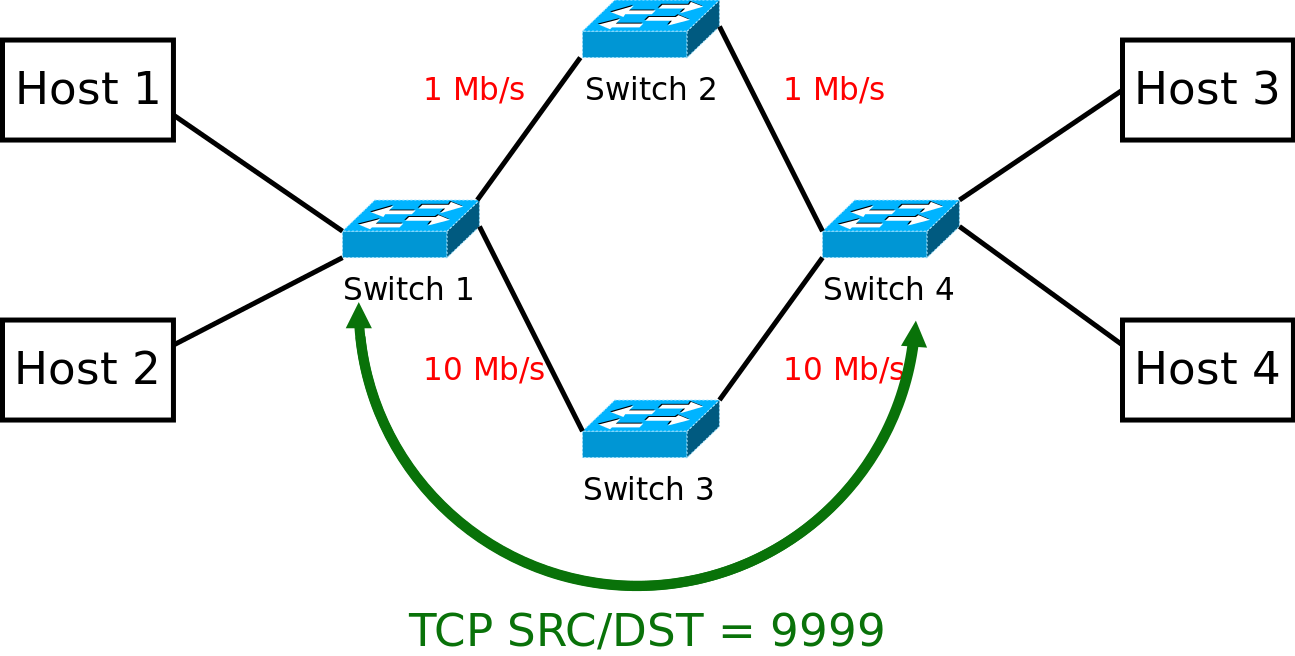
\includegraphics[width=\linewidth]{imagenes/Implementation/mininet_topology_port_slicing.png}
  \caption{Port based slices.}
  \label{fig:port_slicing}
\end{figure}

To fully understand the implementation of this scenario, we need to know how the switch ports are numbered. Every port number is shown in Table \ref{tab:switch_ports}.

\begin{table}
    \centering
    \caption{Port numbering.}
    \vspace{0.1 cm}
    \begin{tabular}{c c}
    \hline
    \rowcolor{lightgray}
    \textbf{Link (A - B)}                        &\textbf{Port number (A - B)}     \\ \hline
    Switch 1 - Host 1                            & 3 - 1                           \\ \hline 
    Switch 1 - Host 2                            & 4 - 1                           \\ \hline 
    Switch 1 - External Host 1                   & 5 - 1                           \\ \hline 
    Switch 2 - Switch 1                          & 1 - 1                           \\ \hline 
    Switch 3 - Switch 1                          & 1 - 2                           \\ \hline 
    Switch 4 - Switch 3                          & 2 - 2                           \\ \hline 
    Switch 4 - Switch 2                          & 1 - 2                           \\ \hline 
    Switch 4 - Host 3                            & 3 - 1                           \\ \hline 
    Switch 4 - Host 4                            & 4 - 1                           \\ \hline 
    Switch 4 - External Host 2                   & 5 - 1                           \\ \hline 
    \end{tabular}
    \label{tab:switch_ports}
\end{table}

We will now go through a brief overview of the necessary commands. To see the full code refer to Appendix \ref{annex:port_slicing}. First of all, we have to create two slices.
\begin{lstlisting}
    fvctl -n add-slice fast_slice tcp:localhost:10001 admin@fastSlice
    fvctl -n add-slice slow_slice tcp:localhost:10002 admin@slowSlice
\end{lstlisting}

Next, we add the flowspaces. As an example, we will show the flowspaces for switch 1.
\begin{lstlisting}
    fvctl -n add-flowspace dpid1_port3_fast_src 1 100 in_port=3,tcp_src=9999 fast=7
    fvctl -n add-flowspace dpid1_port3_fast_dst 1 100 in_port=3,tcp_dst=9999 fast=7
    fvctl -n add-flowspace dpid1_port3_slow 1 1 in_port=3 slow=7
    fvctl -n add-flowspace dpid1_port4_fast_src 1 100 in_port=4,tcp_src=9999 fast=7
    fvctl -n add-flowspace dpid1_port4_fast_dst 1 100 in_port=4,tcp_dst=9999 fast=7
    fvctl -n add-flowspace dpid1_port4_slow 1 1 in_port=4 slow=7
    fvctl -n add-flowspace dpid1_port2 1 100 in_port=2 fast=7
    fvctl -n add-flowspace dpid1_port1 1 1 in_port=1 slow=7
\end{lstlisting}

When it comes to the priorities for each flow, any priority can be used as long as the relativity between them is maintained, i.e., the higher priorities are kept higher than the lower ones.

After configuring every slice and flowspace, we just need to launch FlowVisor and two POX controllers, one listening on port 10001 and the other one on 10002. And that would be it for TCP port slicing. 

Lastly, this is just simple example to get familiar with Mininet, POX, FlowVisor and its syntax. In the next section we will tackle a more complex and involved example now that we know the very basics of network slicing.

\section{IP Address Slicing}
Now, for a more complex scenario, we are going to slice the network depending on the source and destination IP address, see Figure \ref{fig:IP_slicing}. Notice that, before we implement a new scenario, we need to remove the slices created on the previous one. Otherwise the flowspaces and slices will overlap and result on unpredictable behaviour.
\begin{figure}
  \centering
  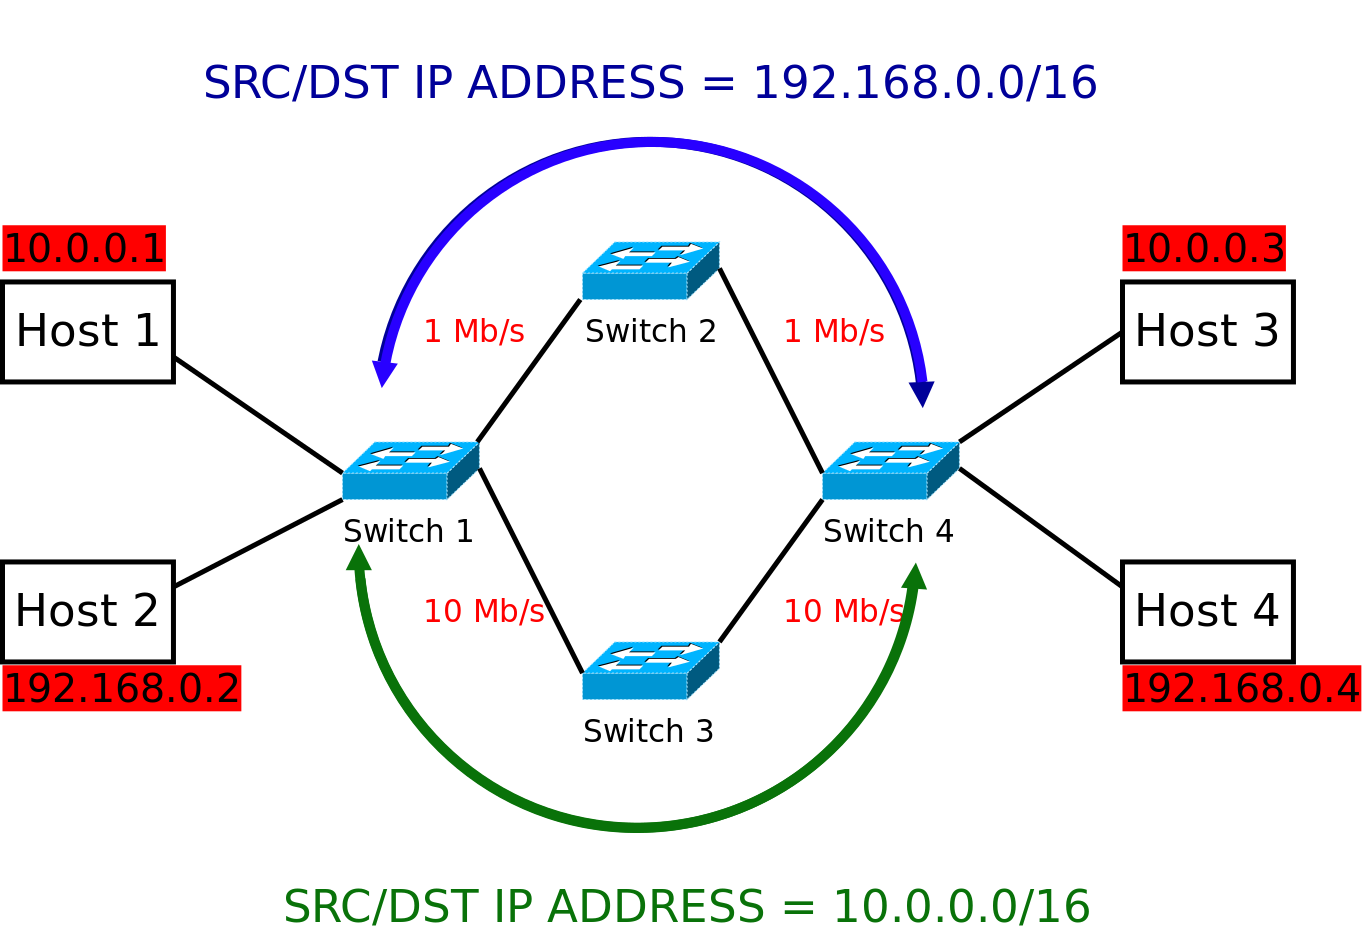
\includegraphics[width=\linewidth]{imagenes/Implementation/mininet_topology_IP_slicing.png}
  \caption{IP address based slices.}
  \label{fig:IP_slicing}
\end{figure}

Similarly to what we did in the previous example, we start by creating the slices. We want to test this scenario later using LoRa packets, thus we name the slices \textit{LoRa} and \textit{Regular}. Furthermore, given that FlowVisor does not have the option to intentionally drop packets, we will create a third slice for this purpose, \textit{DevNull}. This way, whenever we want to intentionally drop packets, we will send them to the DevNull slice. 
\begin{lstlisting}
    fvctl -n add-slice LoRa tcp:localhost:10001 admin@LoRaSlice
    fvctl -n add-slice Regular tcp:localhost:10002 admin@RegularSlice
    fvctl -n add-slice DevNull tcp:localhost:666 admin@DevNull
\end{lstlisting}

In addition, we also want to isolate both subnets, e.g., host 1 cannot communicate with host 4. This is already the case by default because we are using switches. Yet, it is possible to manually add entries to the ARP table so that the switch can route between both subnets. To prevent this, we will actively drop packets that try to leave their original subnet.

Similarly to what we did in the previous example, we will show the flowspaces for switch 1. For the full script, refer to Appendix \ref{annex:ip_slicing}. Also remember that Table \ref{tab:switch_ports} holds the information for the ports of switch 1.
\begin{lstlisting}
    fvctl -n add-flowspace dpid1_LoRa 1 100 nw_src=10.0.0.0/16 LoRa=6
    fvctl -n add-flowspace dpid1_DevNull_LoRa2Regular 1 200 nw_src=10.0.0.0/16,nw_dst=192.168.0.0/16 DevNull=2
    fvctl -n add-flowspace dpid1_DevNull_Regular2LoRa 1 200 nw_dst=192.168.0.0/16,nw_src=10.0.0.0/16 DevNull=2
    fvctl -n add-flowspace dpid1_default 1 1 any Regular=6
    fvctl -n add-flowspace dpid1_DevNull_port1_ARP 1 300 in_port=1,nw_src=10.0.0.0/16,dl_type=0x0806 DevNull=6
    fvctl -n add-flowspace dpid1_Regular_port1 1 1 in_port=1 Regular=6
    fvctl -n add-flowspace dpid1_LoRa_port2_LoRa 1 200 in_port=2,nw_src=10.0.0.0/16 LoRa=6
    fvctl -n add-flowspace dpid1_DevNull_port2 1 1 in_port=2 DevNull=2
\end{lstlisting}

The main ideas behind the flowspaces are:
\begin{itemize}
    \item Drop packets that try to travel between subnets.
    \item Assign packets with \textit{nw\_src=10.0.0.0/16} to LoRa.
    \item Assign ARP packets with \textit{nw\_src=10.0.0.0/16} to LoRa. Technically an ARP packet does not have a network source field, but FlowVisor, due to how it is implemented internally, is able to distinguish between ARP packets based on its source.
    \item Send the rest of the packets to the regular slice.
\end{itemize}

Like we did previously, we now run two POX controllers on ports 10001 and 10002. We do not run a third controller on port 666 because the point of that slice is to drop the packets.

One could think that it should be possible to just send all ARP packets through the same path and reserve the high speed path for actual data packets. The problem with that approach is that, since we are using a learning switch controller, the switches will learn the path to the different hosts through the ARP packets. As a result, the path that is not used for ARP will be completely neglected.

Moreover, we cannot allow the ARP packets to just roam freely through the network because we are using a looped topology. If we do not take care of this loop, the ARP packets will just clog the network and render it useless. 

In conclusion, the flowspaces shown above are the result of many iterations. Mainly due to learning about the different nuances of the topology, as well as the behaviour of the different packets and protocols.


\chapter{Testing}

\cjorge{VOY REVISANDO POR AQUÍ...}

We can now proceed into testing both scenarios and see how they perform when traffic is injected into the network. 

\section{Port Slicing}
For the tests regarding this type of slicing, we have not used real traffic as we just wanted to see if the slicing itself works, instead we have used a tool called Iperf. It allows us to generate either TCP or UDP traffic and it reports back with the bandwidth of the connection. The basic usage of Iperf goes as follows:
\begin{enumerate}
    \item On the end point, call Iperf to listen to a port.
    \begin{lstlisting}
    iperf -s -p <TCP_port_number>
    \end{lstlisting}
    
    \item Now, on a different host, send traffic to the end point.
    \begin{lstlisting}
    iperf -c <ip_address_endpoint> -p <TCP_port_number> -i 1
    \end{lstlisting}
\end{enumerate}

By default, Iperf sends a stream of small TCP packets for 10 seconds. To have a little more granularity, we add the switch \textit{-i 1}. This way we can see the bandwidth of the connection each second, instead of the average of a 10 seconds transmission.

Essentially, by looking at Iperf's bandwidth report, we can tell if the stream of packets is taking the slow or the fast path of the network. This is exactly what we have done, and by looking at Figures \ref{fig:iperf_port_9999} and \ref{fig:iperf_port_8000} we can confirm that the slicing is working as intended:
\begin{itemize}
    \item When the TCP connection is on port 9999, the bandwidth reported is \SIrange[per-mode=symbol]{7}{17}{\mega\bit\per\second}, which means the packets are taking the fast path. 
    \item Likewise, if the port is different from 9999, e.g, port 8000, the packets take the slow route and we see a bandwidth of \SIrange[per-mode=symbol]{1}{3}{\mega\bit\per\second}.
\end{itemize}

\begin{figure}
  \centering
  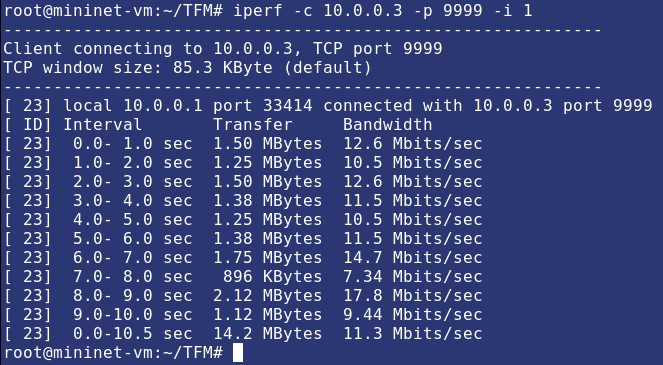
\includegraphics[width=\linewidth]{imagenes/Testing/port_slicing_iperf_fast.png}
  \caption{Iperf's bandwidth report of a TCP connection to port 9999, from host 1 to host 3.}
  \label{fig:iperf_port_9999}
\end{figure}

\begin{figure}
  \centering
  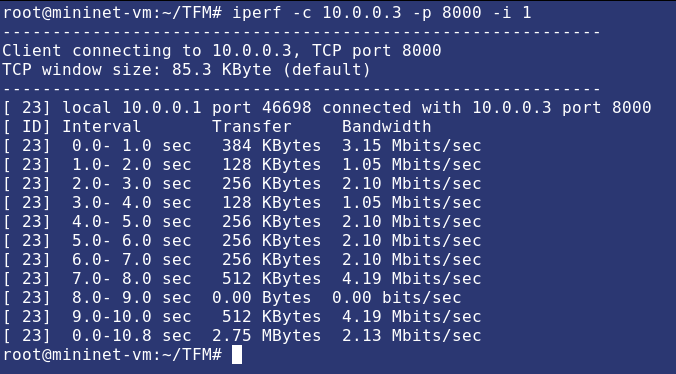
\includegraphics[width=\linewidth]{imagenes/Testing/port_slicing_iperf_slow.png}
  \caption{Iperf's bandwidth report of a TCP connection to port 8000, from host 1 to host 3.}
  \label{fig:iperf_port_8000}
\end{figure}

\subsection{Analysis of the Results}
While the bandwidth measurements are not entirely accurate, the margin between the tests is clear enough to warrant the correct slicing implementation, i.e. the packets take the intended path.

\cjorge{Yo cambiaría un poco el enfoque. VLAN usa port slicing usando el concepto de puerto de switch, no puerto de TCP/UDP. Así que diría que hace algo similar y por tanto el concepto no es nuevo. Pero igual, igual, no es.}

As it has been mentioned before, this type of network slicing is nothing new. Port based slicing is exactly what VLANs do in traditional networks and, in fact, have been widely used for many years. Nevertheless, it is still important to prove that port based slicing is still possible in the new network paradigm of SDNs.

\section{IP Address Slicing}
\subsection{Preparation}
In this scenario, we have performed a more advanced and complex test involving external hosts. While Iperf would have sufficed, we have opted for a test that closer resembles a real production environment, illustrated by Figured \ref{fig:topology_LoRa}. The physical setup is shown in Figure \ref{fig:LoRa_setup}. The main elements for this test are:
\begin{itemize}
    \item \textbf{LoRa mote}. It will broadcast packets over air using the LoRa protocol.
    \item \textbf{LoRa gateway}. Responsible for capturing the LoRa packets transmitted over air and forwarding them \cjorge{to the LoRaWAN network and application servers through the virtual Mininet network, which publish the messages using MQTT. Y QUITARÍA LO QUE SIGUE EN ESTE PÁRRAFO.}to the MQTT client through the virtual Mininet network. 
    \item \textbf{MQTT client}. If everything works correctly, it should receive the packets originally sent by the LoRa mote. In addition, these packets should traverse the Mininet network through the slow path. 
\end{itemize}

\cjorge{En esta figura faltan los servidores de red y aplicación LoRaWAN...}

\begin{figure}
  \centering
  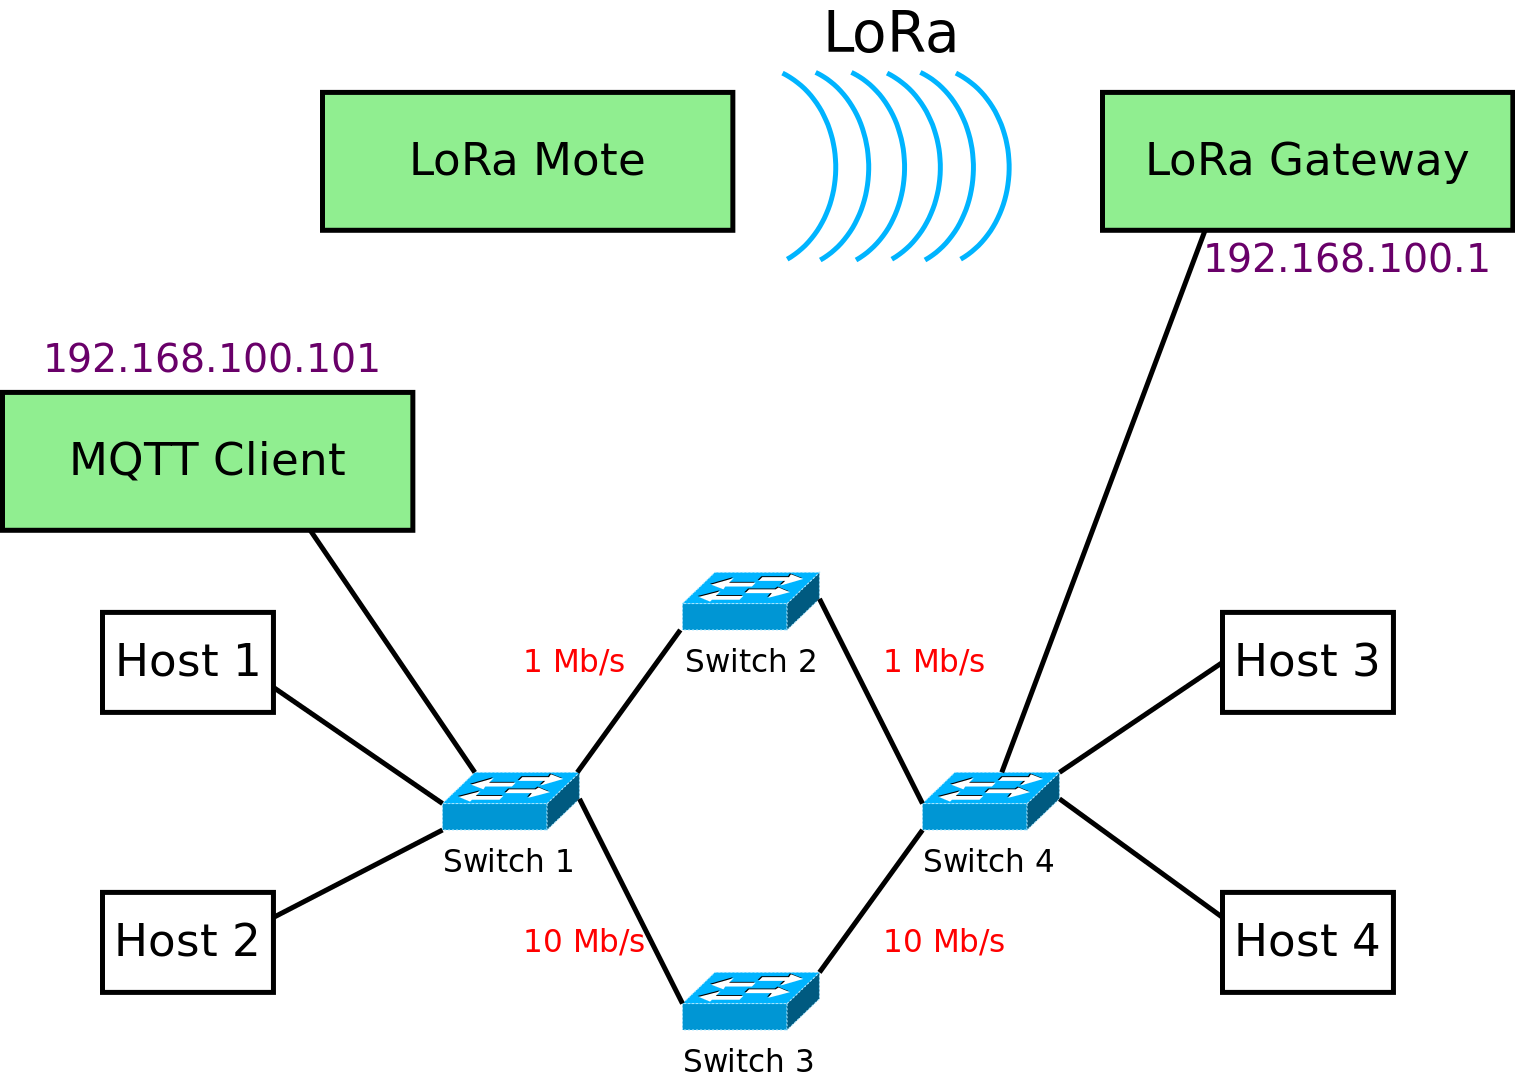
\includegraphics[width=\linewidth]{imagenes/Testing/mininet_topology_LoRa.png}
  \caption{Testing scenario for IP address slicing.}
  \label{fig:topology_LoRa}
\end{figure}

As for the MQTT client, we will use \textit{Mosquitto}.
\begin{lstlisting}
    mosquitto_sub -h localhost -t "gateway/#" -v 
\end{lstlisting}

Where:
\begin{itemize}
    \item \textbf{localhost}. Host where the messages are stored.
    \item \textbf{gateway/\#}. Topic we wish to subscribe to.
\end{itemize}

In addition, due to using Mininet within a virtual machine, the MQTT client must go through the physical Ethernet interface of the Mininet network host, which is not possible if said Ethernet interface does not belong to the same subnet, i.e., 192.168.0.0/16. There are several ways to accomplish this. We have opted to edit the configuration file at \textit{/etc/dhcpcd.conf}, adding the following lines at the end of the file:
\begin{lstlisting}
    interface eno1
    static ip_address=192.168.100.50/16
\end{lstlisting}

Where:
\begin{itemize}
    \item \textbf{eno1}. Name of our Ethernet interface on the Mininet network host.
    \item \textbf{192.168.100.50/16}. IP assigned to the interface. It can be any valid IP within the subnet as long as it is not already taken.
\end{itemize}

Lastly, for the test to be considered successful, every LoRa packet must be received at the MQTT client and packets must go through the slow path. To verify that this is the case, we will use the tool \textit{Tshark}, which is a terminal based packet sniffer.

\begin{figure}
  \centering
  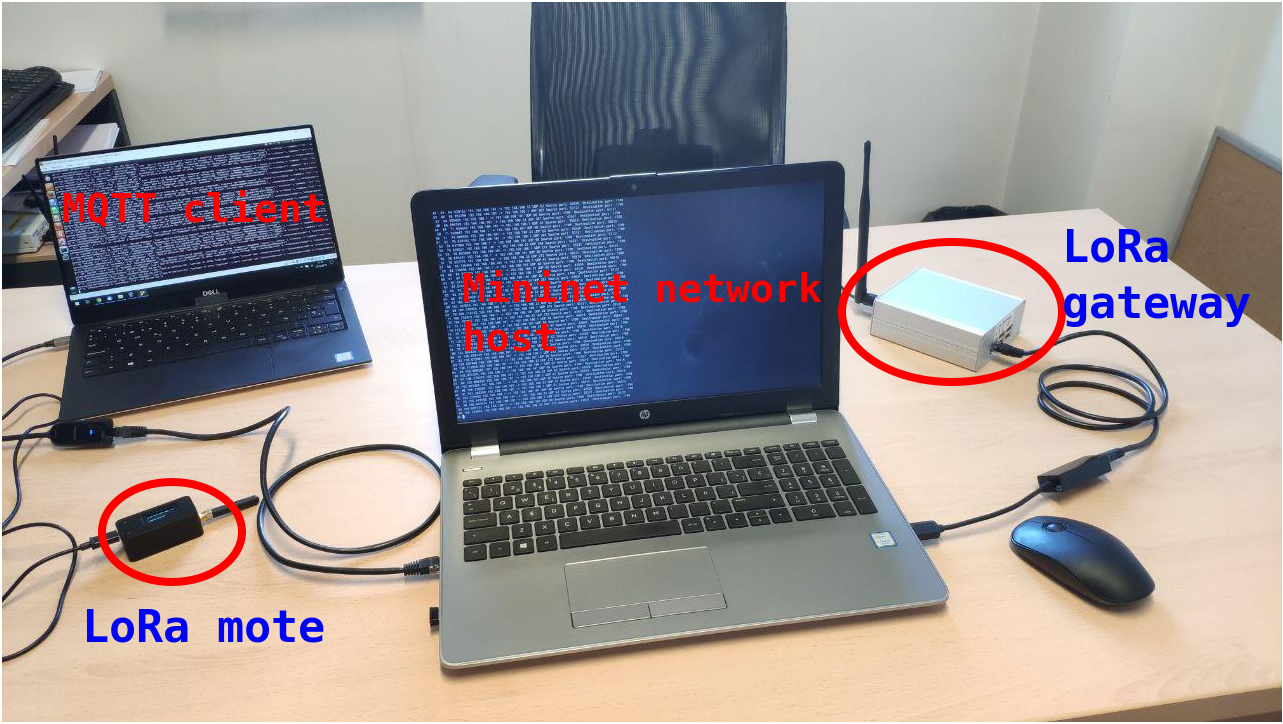
\includegraphics[width=\linewidth]{imagenes/Testing/lora_setup.png}
  \caption{Setup of the physical test components.}
  \label{fig:LoRa_setup}
\end{figure}

\subsection{Analysis of the Results}
Judging by Figure \ref{fig:mosquitto}, it looks like everything is working as expected. The LoRa packages are being forwarded correctly by the LoRa gateway and arriving at the MQTT client. Nevertheless, we still need to ensure that they are taking the correct path, as that is the actual point of this test. Thankfully, Figure \ref{fig:LoRa_tshark} shows that the packets are going through switch 2, which is the correct path, so everything is working correctly.

\begin{figure}
  \centering
  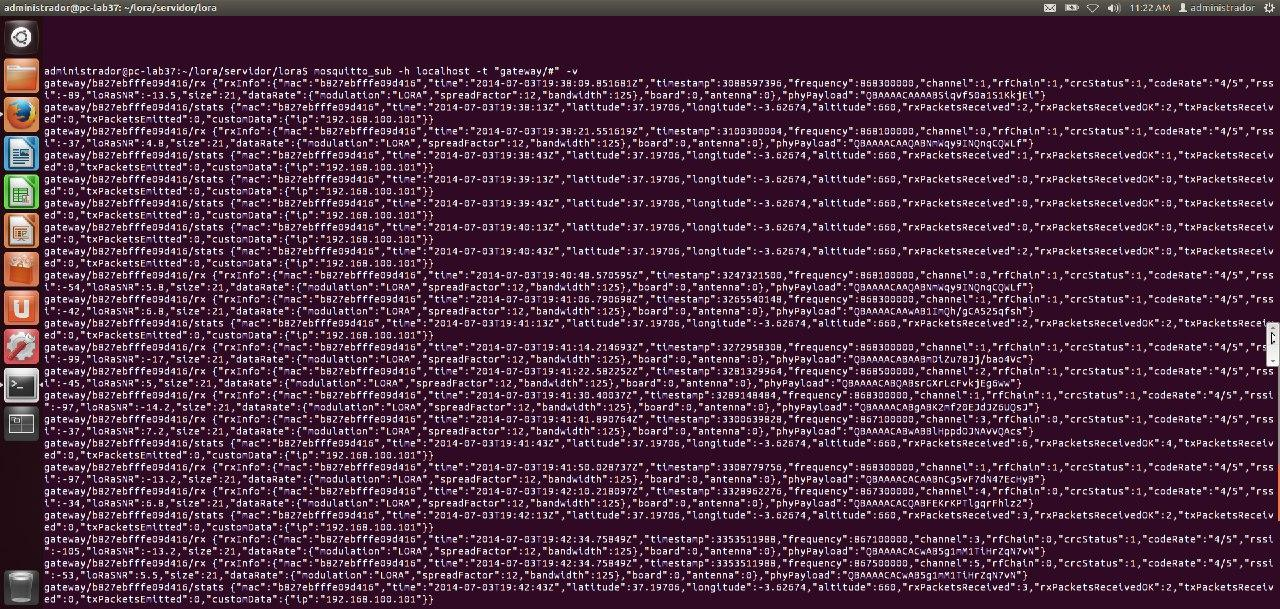
\includegraphics[width=\linewidth]{imagenes/Testing/mosquitto_packets.png}
  \caption{Packets shown on the MQTT client.}
  \label{fig:mosquitto}
\end{figure}

\begin{figure}
  \centering
  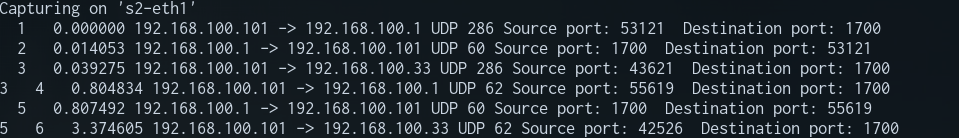
\includegraphics[width=\linewidth]{imagenes/Testing/tshark-LoRa.png}
  \caption{Packets sniffed by Tshark on switch 2.}
  \label{fig:LoRa_tshark}
\end{figure}

\cjorge{No recuerdo si has comentado que LoRaWAN se usa para IoT... haz algún comentario en este sentido, porque el lector puede no conocer LoRaWAN previamente.}

In this particular case, the slices help us isolate IoT traffic and send it through a slower path of the network. This way, we leave the faster path available for other types of traffic that require a higher bandwidth.

But, if we look past our example, there are many other ways in which it could benefit a real production network: providing traffic engineering for QoS, isolating traffic between different services or enabling a production network to be used as testbed for a different service among others possibilities. All in all, there is definitely a plethora of use-cases. 
\chapter{Conclusions}
First off, software defined networks are extremely useful by themselves. They provide us with much better scalability, they deal with the issue of heterogeneous hardware and compatibility across the same network and offer a broader network view to perform traffic engineering. 

Furthermore, an SDN hypervisor that sits between the physical devices and the OpenFlow controllers proves to be a very powerful tool as well. It simplifies the deployment of OpenFlow controllers while, at the same time, dealing with the problem of adaptability in complex networks and enabling a feasible and maintainable way to perform network virtualization or network slicing.

Speaking of network virtualization, its real world applications are endless, as pointed out at the end of the previous chapter. It is definitely something to consider when designing a network because, when used correctly, it provides the network with great flexibility, scalability, adaptability and efficiency.

On the other hand, the development of open source hypervisors seems to have reached a full stop. FlowVisor is the only one available at the time of writing this document and it has not seen an update to its code base since August 2013. However, the technique itself is very much still in use, as it is a prevalent feature of the up and coming 5G cellular networks.   

In summary, network slicing is a very powerful technique and definitely has a bright future in the coming generation of cellular networks. Yet, it looks like said future lies in the private industry, as opposed to open source.

\section{Future Work}
If this project were to be continued, the first thing we would do would be to test both implementations in a real network with physical OpenFlow devices. Testing using a virtual network is acceptable, but there might be problems that only arise once deployed in a physical one.

On a different note, exploring different ways of slicing the network would also be interesting. So far we have tried TCP port and IP address slicing, but FlowVisor offers a few more parameters to choose from.
\begin{itemize}
    \item MAC address.
    \item Ethernet protocol.
    \item Physical switch port.
    \item Network protocol.
    \item ToS/DSCP IPv4 header.
\end{itemize}

Overall, this project can definitely be extended and improved upon, although it has managed to address the main points that we aimed to cover.


%\nocite{*}
\bibliographystyle{ieeetr}
\bibliography{bibliography}

\begin{appendices}
\chapter{Mininet Topology} \label{annex:mininet}
The is the Python code used to generate the Mininet topology. It includes:
\begin{itemize}
    \item Four virtual switches.
    \item Four virtual hosts.
    \item Two external interfaces.
\end{itemize}

\begin{lstlisting}[language=Python]
#!/usr/bin/python

# Add mininet's directory to path.
import sys
sys.path.append('/home/mininet/mininet')

from mininet.topo import Topo
from mininet.net import Mininet
from mininet.link import Intf, TCLink
from mininet.node import RemoteController
from mininet.cli import CLI
from mininet.log import setLogLevel, info


class FVTopo(Topo):
	"""Based on:
	https://github.com/onstutorial/onstutorial/blob/master/flowvisor_scripts/flowvisor_topo.py"""

	def __init__(self):
		# Initialize topology.
		Topo.__init__(self)

		N_switches = 4
		N_hosts = 4

		# Create template host, switch, and link.
		normal_link_config = {'bw': 1}
		LoRa_link_config = {'bw': 10}
		host_link_config = {}

		# Create switch nodes.
		for i in range(1, N_switches + 1):
			sconfig = {'dpid': "%016x" % (i)}
			self.addSwitch('s%d' % (i), **sconfig)

		# Create host nodes.
		for i in range(1, N_hosts + 1):
			if i%2 == 0:
				hconfig = {'inNamesapce':True, 'ip': "192.168.0.%d" % (i)}
				self.addHost('h%d' % (i), **hconfig)
			if i%2 != 0:
				hconfig = {'inNamesapce':True, 'ip': "10.0.0.%d" % (i)}
				self.addHost('h%d' % (i), **hconfig)

		# Add switch links.
		self.addLink('s1', 's2', **normal_link_config)
		self.addLink('s2', 's4', **normal_link_config)
		self.addLink('s1', 's3', **LoRa_link_config)
		self.addLink('s3', 's4', **LoRa_link_config)

		# Add host links.
		self.addLink('h1', 's1', **host_link_config)
		self.addLink('h2', 's1', **host_link_config)
		self.addLink('h3', 's4', **host_link_config)
		self.addLink('h4', 's4', **host_link_config)


def run_fvtopo():
	# Create topology.
	net = Mininet(topo = FVTopo(), controller = RemoteController, autoSetMacs = True, autoStaticArp = False, link = TCLink)

	# Add external interface.
	intfName0= 'eth0'
	intfName1= 'eth1'

	switch1 = net.switches[0]
	info('*** Adding hardware interface', intfName0, 'to switch', switch1.name, '\n')
	_intf = Intf(intfName0, node=switch1)

	switch4 = net.switches[-1]
	info('*** Adding hardware interface', intfName1, 'to switch', switch4.name, '\n')
	_intf = Intf(intfName1, node=switch4)

	# Run it.
	net.start()
	CLI(net)
	net.stop()


if __name__ == '__main__':
	setLogLevel('info')
	run_fvtopo()


# Preserve the --custom functionality.
topos = {'fvtopo': FVTopo}
\end{lstlisting}
\chapter{TCP Port Slicing} \label{annex:port_slicing}
Bash script to quickly set up networking slicing based on TCP ports.

\begin{lstlisting}[language=bash]
# This script creates two slices: fast and slow traffic.


# Create both slices.
fvctl -n add-slice fast tcp:localhost:10001 admin@fastSlice
fvctl -n add-slice slow tcp:localhost:10002 admin@slowSlice

# Add flowspaces for switch 1.
fvctl -n add-flowspace dpid1_port3-fast_src 1 100 in_port=3,dl_type=0x0800,nw_proto=6,tp_src=9999 fast=7  # Priority 100.
fvctl -n add-flowspace dpid1_port3-fast_dst 1 100 in_port=3,dl_type=0x0800,nw_proto=6,tp_dst=9999 fast=7
fvctl -n add-flowspace dpid1_port3-slow 1 1 in_port=3 slow=7
fvctl -n add-flowspace dpid1_port4-fast_src 1 100 in_port=4,dl_type=0x0800,nw_proto=6,tp_src=9999 fast=7
fvctl -n add-flowspace dpid1_port4-fast_dst 1 100 in_port=4,dl_type=0x0800,nw_proto=6,tp_dst=9999 fast=7
fvctl -n add-flowspace dpid1_port4-slow 1 1 in_port=4 slow=7
fvctl -n add-flowspace dpid1_port2-fast 1 100 in_port=2 fast=7
fvctl -n add-flowspace dpid1_port1-fast 1 1 in_port=1 slow=7

# Add flowspaces for switch 2.
fvctl -n add-flowspace dpid2 2 1 any slow=7

# Add flowspaces for switch 3.
fvctl -n add-flowspace dpid3 3 100 any fast=7 

# Add flowspaces for switch 4.
fvctl -n add-flowspace dpid4_port3-fast_src 4 100 in_port=3,dl_type=0x0800,nw_proto=6,tp_src=9999 fast=7
fvctl -n add-flowspace dpid4_port3-fast_dst 4 100 in_port=3,dl_type=0x0800,nw_proto=6,tp_dst=9999 fast=7
fvctl -n add-flowspace dpid4_port3-slow 4 1 in_port=3 slow=7
fvctl -n add-flowspace dpid4_port4-fast_src 4 100 in_port=4,dl_type=0x0800,nw_proto=6,tp_src=9999 fast=7
fvctl -n add-flowspace dpid4_port4-fast_dst 4 100 in_port=4,dl_type=0x0800,nw_proto=6,tp_dst=9999 fast=7
fvctl -n add-flowspace dpid4_port4-slow 4 1 in_port=4 slow=7
fvctl -n add-flowspace dpid4_port2-fast 4 100 in_port=2 fast=7
fvctl -n add-flowspace dpid4_port4-fast 4 1 in_port=1 slow=7
\end{lstlisting}
\chapter{IP Address Slicing} \label{annex:ip_slicing}
Bash script to quickly set up networking slicing based on IP address.

\begin{lstlisting}[language=bash]
# This script creates three slices: LoRa, Regular traffic and a DevNull slice to drop packets.

# Create both slices.
fvctl -n add-slice LoRa tcp:localhost:10001 admin@LoRaSlice
fvctl -n add-slice Regular tcp:localhost:10002 admin@RegularSlice
fvctl -n add-slice DevNull tcp:localhost:666 admin@DevNull


# Add flowspaces for switch 1.
fvctl -n add-flowspace dpid1_LoRa 1 100 nw_src=10.0.0.0/16 LoRa=6

fvctl -n add-flowspace dpid1_DevNull_LoRa2Regular 1 200 nw_src=10.0.0.0/16,nw_dst=192.168.0.0/16 DevNull=2
fvctl -n add-flowspace dpid1_DevNull_Regular2LoRa 1 200 nw_dst=192.168.0.0/16,nw_src=10.0.0.0/16 DevNull=2

fvctl -n add-flowspace dpid1_default 1 1 any Regular=6

fvctl -n add-flowspace dpid1_DevNull_port1_ARP 1 300 in_port=1,nw_src=10.0.0.0/16,dl_type=0x0806 DevNull=6
fvctl -n add-flowspace dpid1_Regular_port1 1 1 in_port=1 Regular=6

fvctl -n add-flowspace dpid1_LoRa_port2_LoRa 1 200 in_port=2,nw_src=10.0.0.0/16 LoRa=6
fvctl -n add-flowspace dpid1_DevNull_port2 1 1 in_port=2 DevNull=2


# Add flowspaces for switch 2.
fvctl -n add-flowspace dpid2_DevNull_ARP 2 300 nw_src=10.0.0.0/16,dl_type=0x0806 DevNull=6
fvctl -n add-flowspace dpid2 2 1 any Regular=6


# Add flowspaces for switch 3.
fvctl -n add-flowspace dpid3_DevNull_ARP 3 300 nw_src=192.168.0.0/16,dl_type=0x0806 DevNull=6
fvctl -n add-flowspace dpid3 3 100 nw_src=10.0.0.0/16 LoRa=6
fvctl -n add-flowspace dpid3_DevNull 3 1 any DevNull=2


# Add flowspaces for switch 4.
fvctl -n add-flowspace dpid4_LoRa 4 100 nw_src=10.0.0.0/16 LoRa=6

fvctl -n add-flowspace dpid4_DevNull_LoRa2Regular 4 200 nw_src=10.0.0.0/16,nw_dst=192.168.0.0/16 DevNull=2
fvctl -n add-flowspace dpid4_DevNull_Regular2LoRa 4 200 nw_dst=192.168.0.0/16,nw_src=10.0.0.0/16 DevNull=2

fvctl -n add-flowspace dpid4_default 4 1 any Regular=6

fvctl -n add-flowspace dpid4_DevNull_port1_ARP 4 300 in_port=1,nw_src=10.0.0.0/16,dl_type=0x0806 DevNull=6
fvctl -n add-flowspace dpid4_Regular_port4 4 1 in_port=1 Regular=6

fvctl -n add-flowspace dpid4_LoRa_port2_LoRa 4 200 in_port=2,nw_src=10.0.0.0/16 LoRa=6
fvctl -n add-flowspace dpid4_DevNull_port2 4 1 in_port=2 DevNull=2
\end{lstlisting}
\end{appendices}

\chapter*{}
\thispagestyle{empty}

\end{document}
